% --- SLIDE 9: Connecting Degenerate Strings to DAGs ---
\begin{frame}{From Degenerate Strings to Weighted DAGs}
    \framesubtitle{A New Perspective}

    Recall our degenerate string $X$:
    \begin{figure}[h!]
        \centering
        % Usa la figura della stringa degenere che hai già definito
        \begin{tabular}{c@{\hskip 0.5em}c@{\hskip 0.5em}c@{\hskip 0.5em}c@{\hskip 0.5em}c}
            $X = $                                                                           & $\Bigg\{\,\begin{matrix}\texttt{A}\\\texttt{C}\\\texttt{G}\end{matrix}\,\Bigg\}$ &
            $\Bigg\{\,\begin{matrix}\texttt{A}\\\texttt{T}\end{matrix}\,\Bigg\}$             &
            $\Bigg\{\,\begin{matrix}\texttt{T}\\\texttt{C}\\\texttt{A}\end{matrix}\,\Bigg\}$ &
            $\Bigg\{\,\begin{matrix}\texttt{A}\\\texttt{G}\end{matrix}\,\Bigg\}$                                                                                                                        \\
                                                                                             & $X_1$                                                                            & $X_2$ & $X_3$ & $X_4$
        \end{tabular}
    \end{figure}

    \uncover<2->{
        \begin{block}{Key Idea}
            We can model queries on $X$ by constructing a specific node-weighted Directed Acyclic Graph (DAG) $G_c$ for a target character $c$.
        \end{block}
    }

    \uncover<3->{
        \begin{itemize}
            \item<3-> \textbf{Vertices $V_c$}: Source $s$ + one node $v_{k,a}$ for each character $a \in X_k$ at each position $k$.
            \item<4-> \textbf{Weights $w_c$}: $w_c(s)=0$. $w_c(v_{k,a}) = 1$ if $a = c$, else $0$. (Highlights occurrences of $c$).
            \item<5-> \textbf{Edges $E_c$}: Connect $s$ to $k=1$. Connect all $v_{k,a}$ to all $v_{k+1,b}$. (Represents sequence adjacency).
        \end{itemize}
    }

\end{frame}

% --- SLIDE 10: Path Weight Aggregation: The O-Set Definition ---
\begin{frame}{Path Weight Aggregation: The $\mathcal{O}$-Set}
    \framesubtitle{Capturing All Path Weights}
    Given a path $P=(v_0=s, \dots, v_k=v)$ we define $W(P) = \sum_{j=1}^{k} w(v_j)$
    \begin{alertblock}{Goal}
        Characterize the set of \alert{all possible distinct} cumulative path weights arriving at each node.
    \end{alertblock}
    % \vspace{1em}
    \pause
    \begin{block}{$\mathcal{O}$-Set Definition (Recursive)}
        \begin{itemize}
            \item \textbf{Base Case (Source):} $\mathcal{O}_s = \{0\}$
            \item \textbf{Recursive Step ($v \neq s$):}
                  \[ \mathcal{O}_v = \bigcup_{u \in Pred(v)} \{ y + w(v) \mid y \in \mathcal{O}_u \} = \{ W(P) \mid P \in Path(s, v) \}  \]
                  Keep only \alert{distinct} values. Store as a sorted sequence.
        \end{itemize}
    \end{block}
    % The set $\mathcal{O}_v$ contains \emph{exactly} the weights $W(P)$ for all paths $P$ from source $s$ to $v$.
    % \[ \mathcal{O}_v = \{ W(P) \mid P \in Path(s, v) \} \]

\end{frame}

% --- SLIDE 11: O-Set Construction Example ---
\begin{frame}{$\mathcal{O}$-Set Construction Example}
    \framesubtitle{Visualizing the Recursive Definition}
    \vspace{-0.5em}
    \begin{figure}[hbtp]
        % \centering
        % Replace TikZ with sequential images
        \only<1>{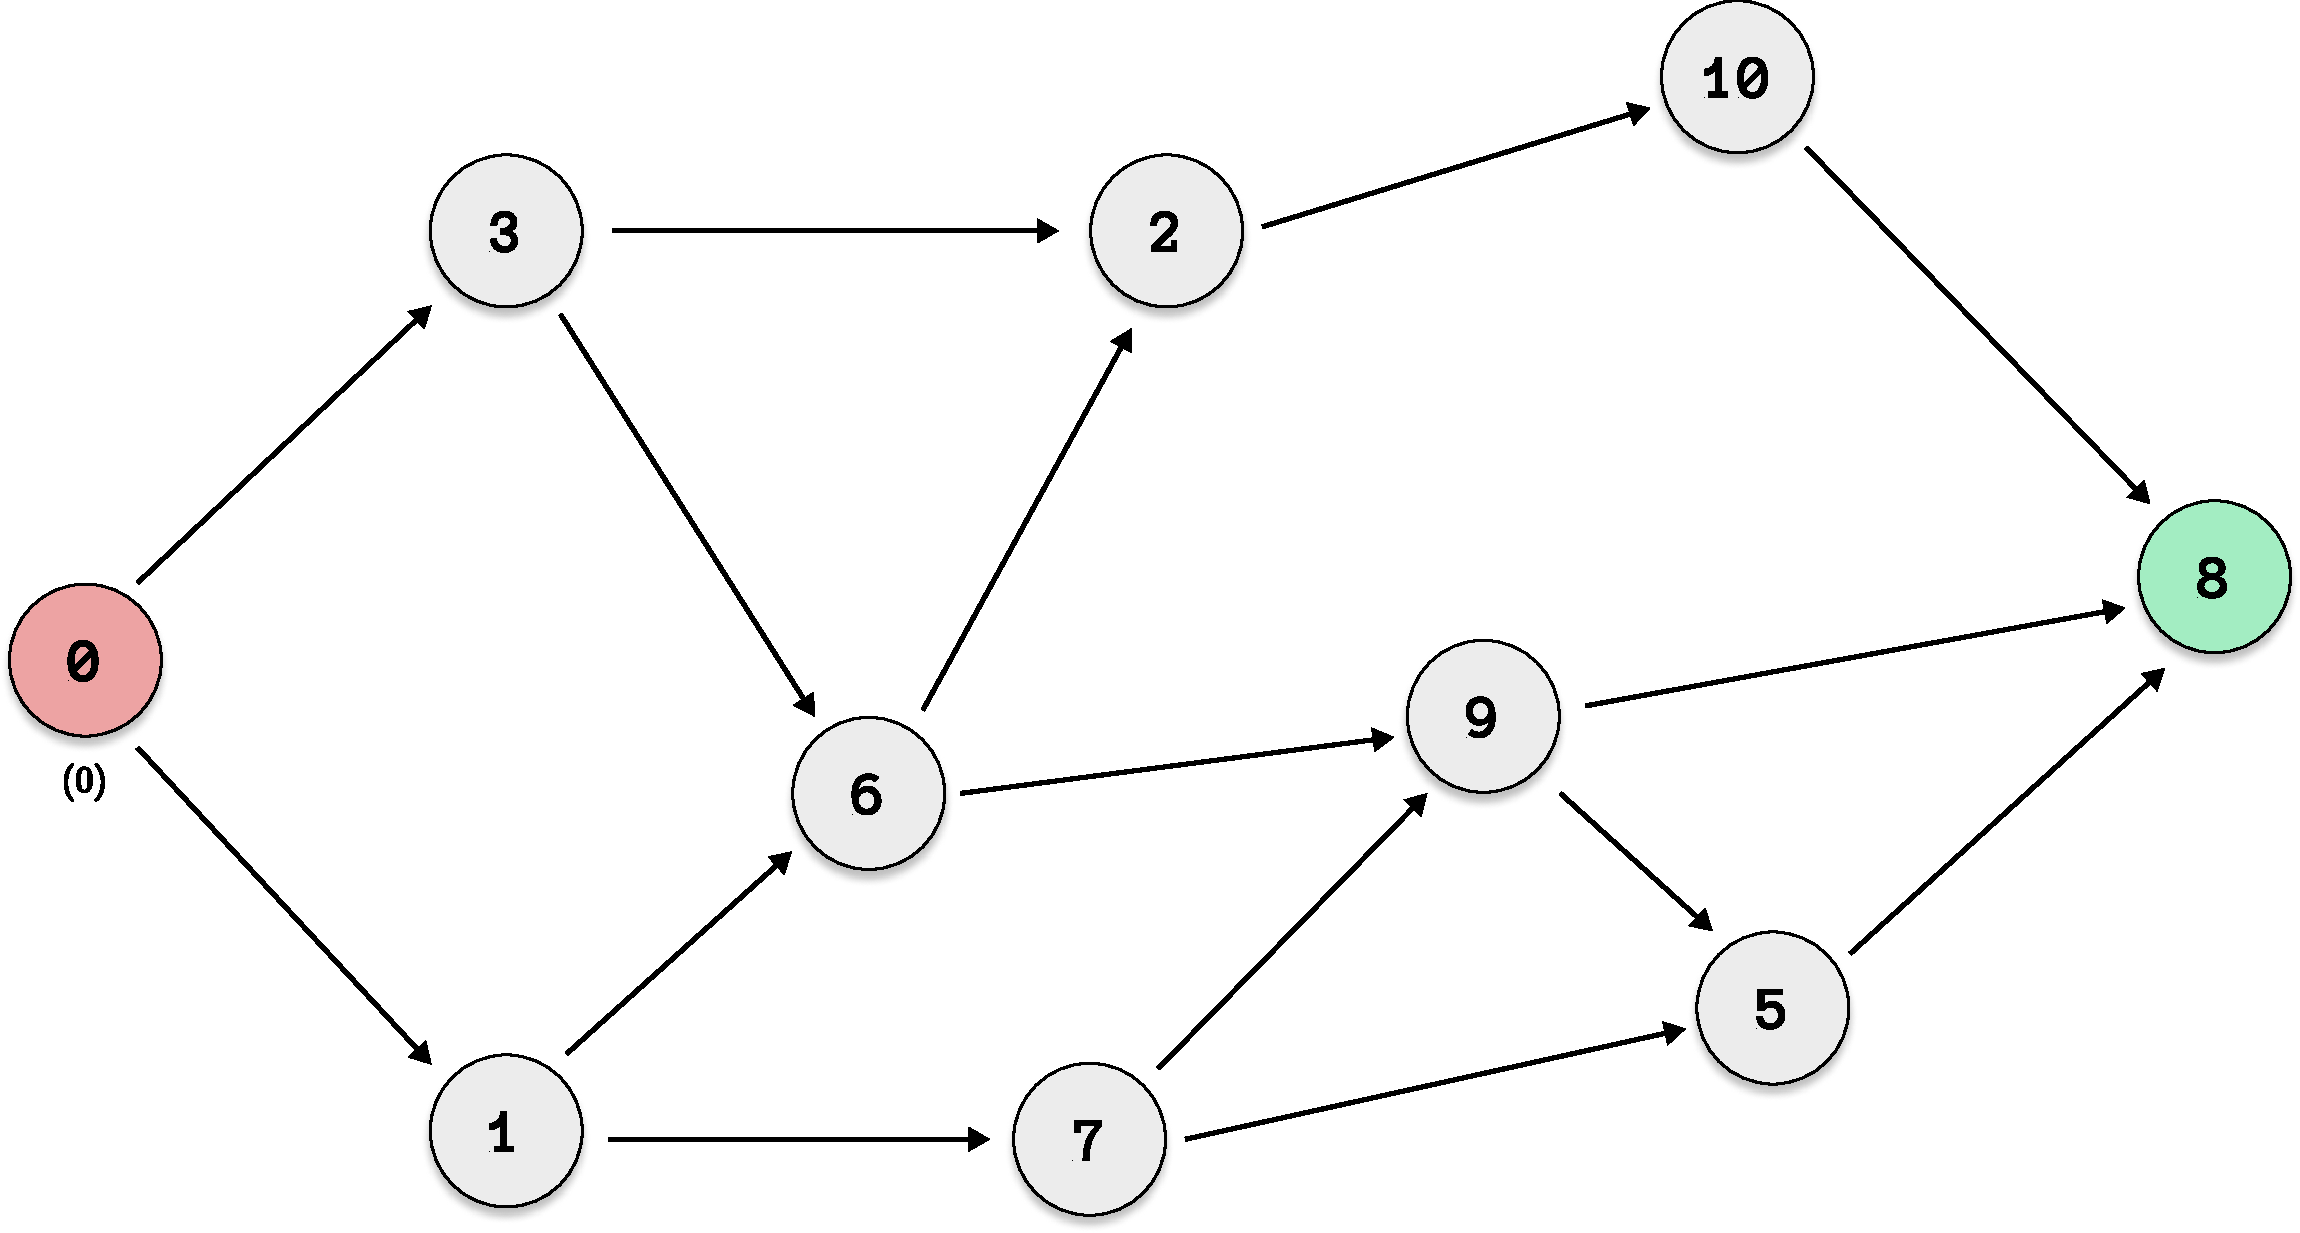
\includegraphics[width=0.85\textwidth]{assets/dag_explicit1.pdf}}
        % \only<2>{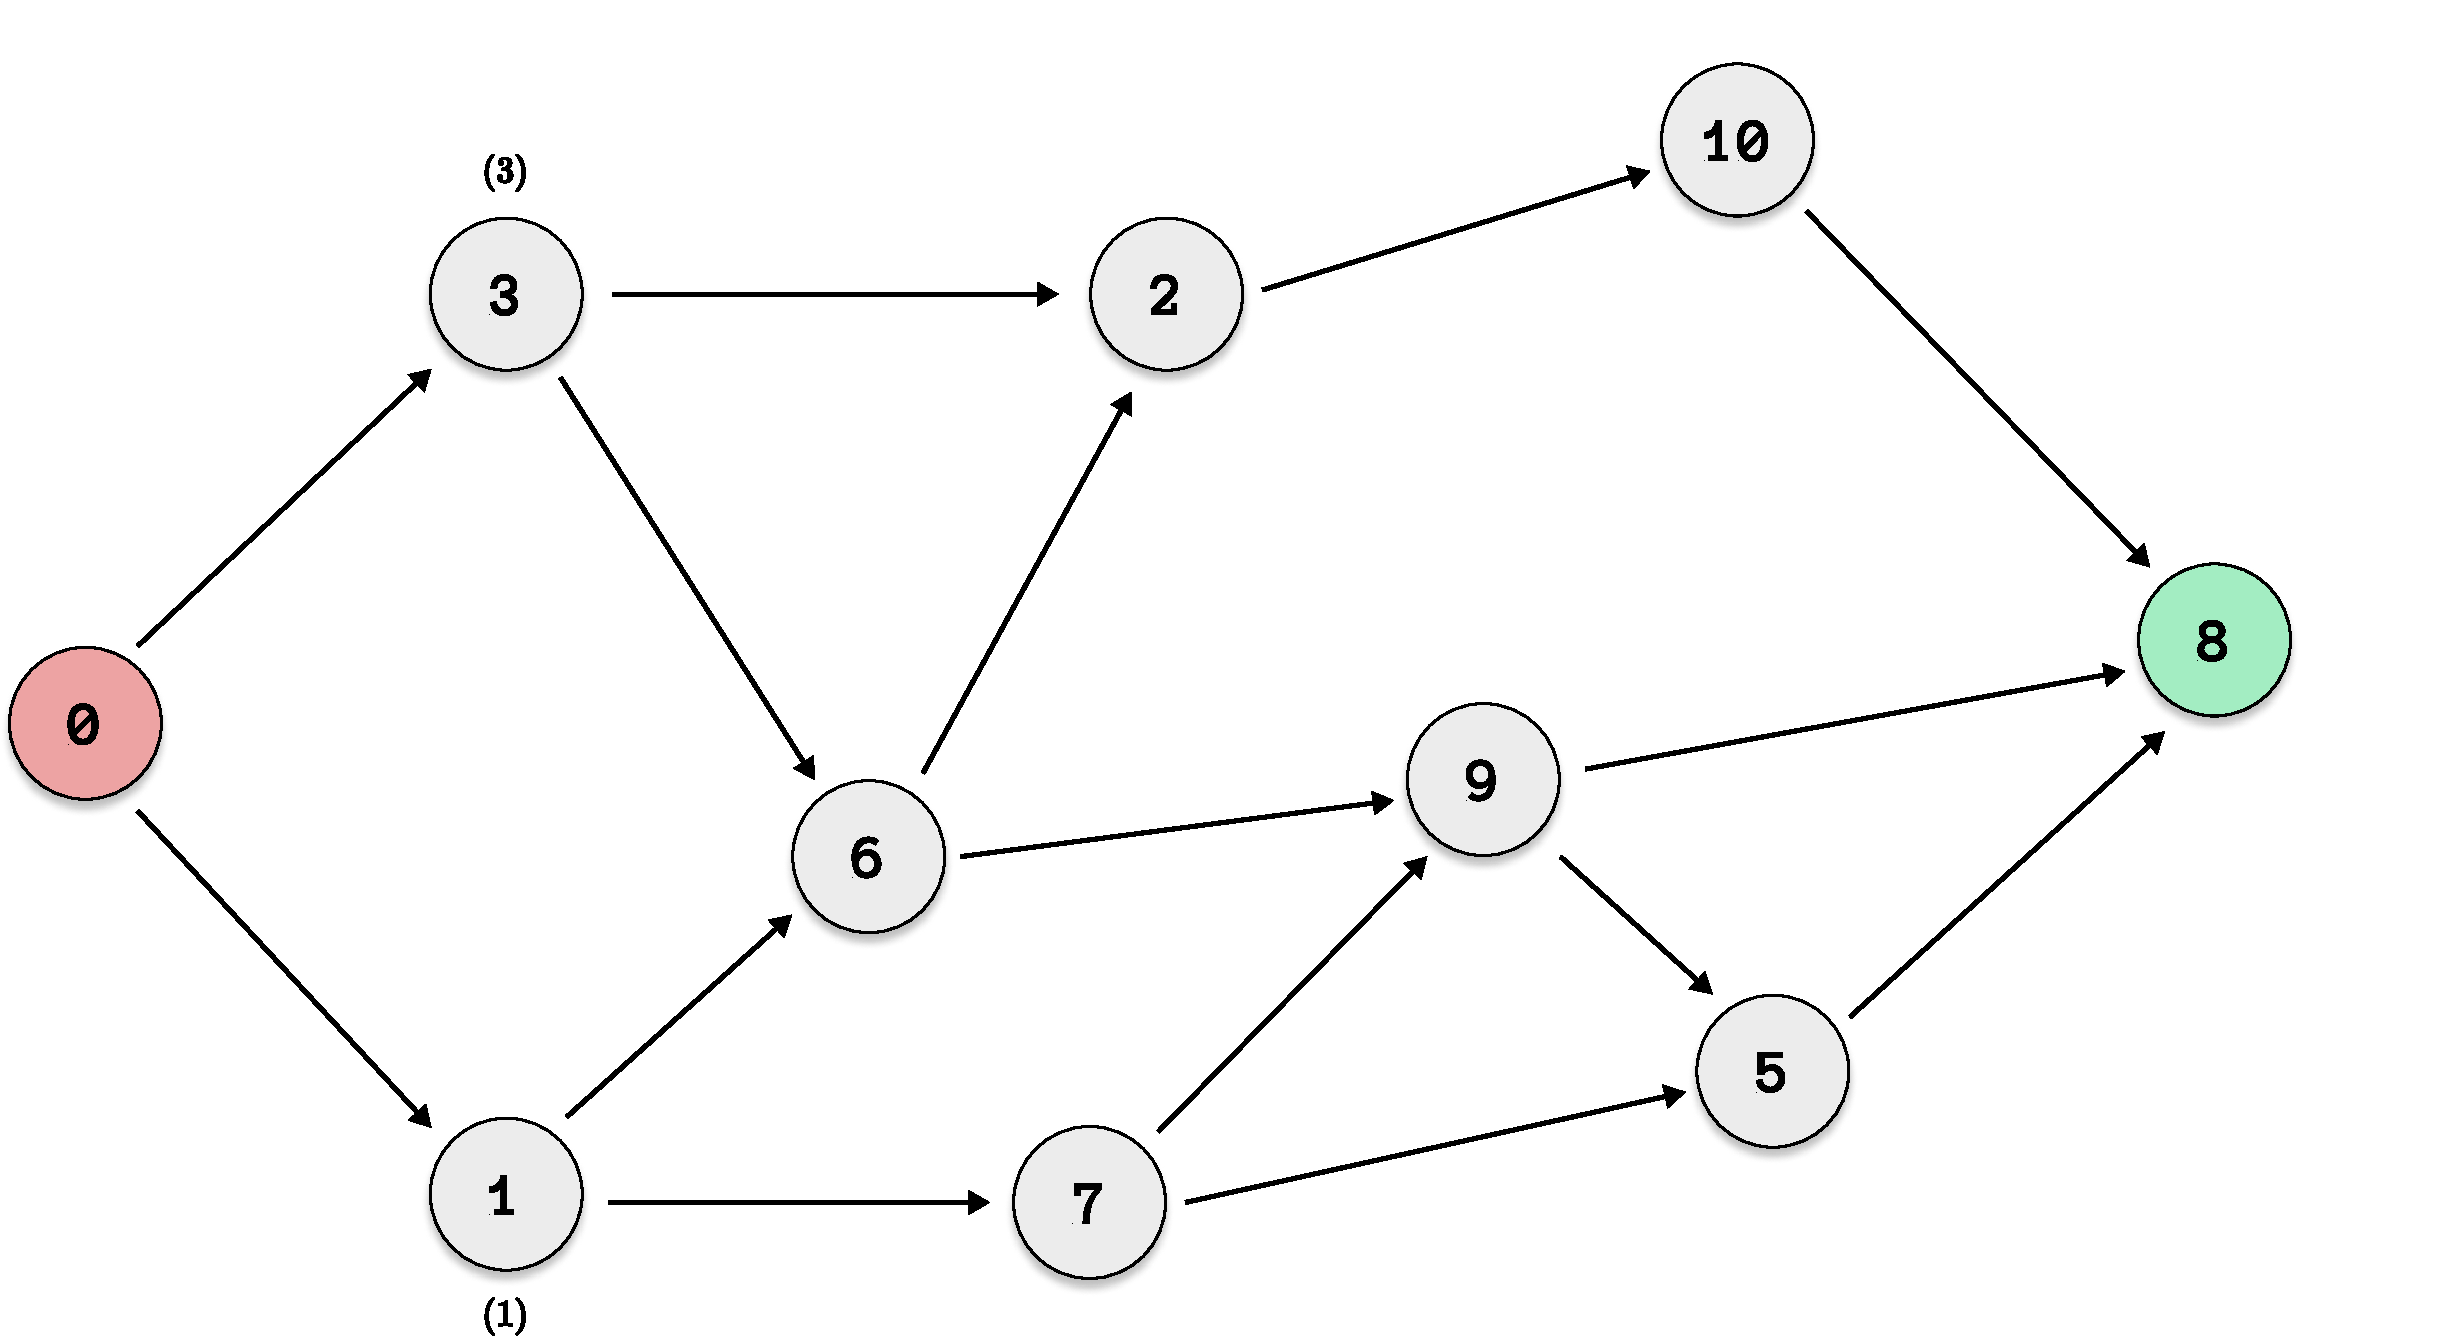
\includegraphics[width=0.85\textwidth]{assets/dag_explicit2.pdf}}
        \only<2>{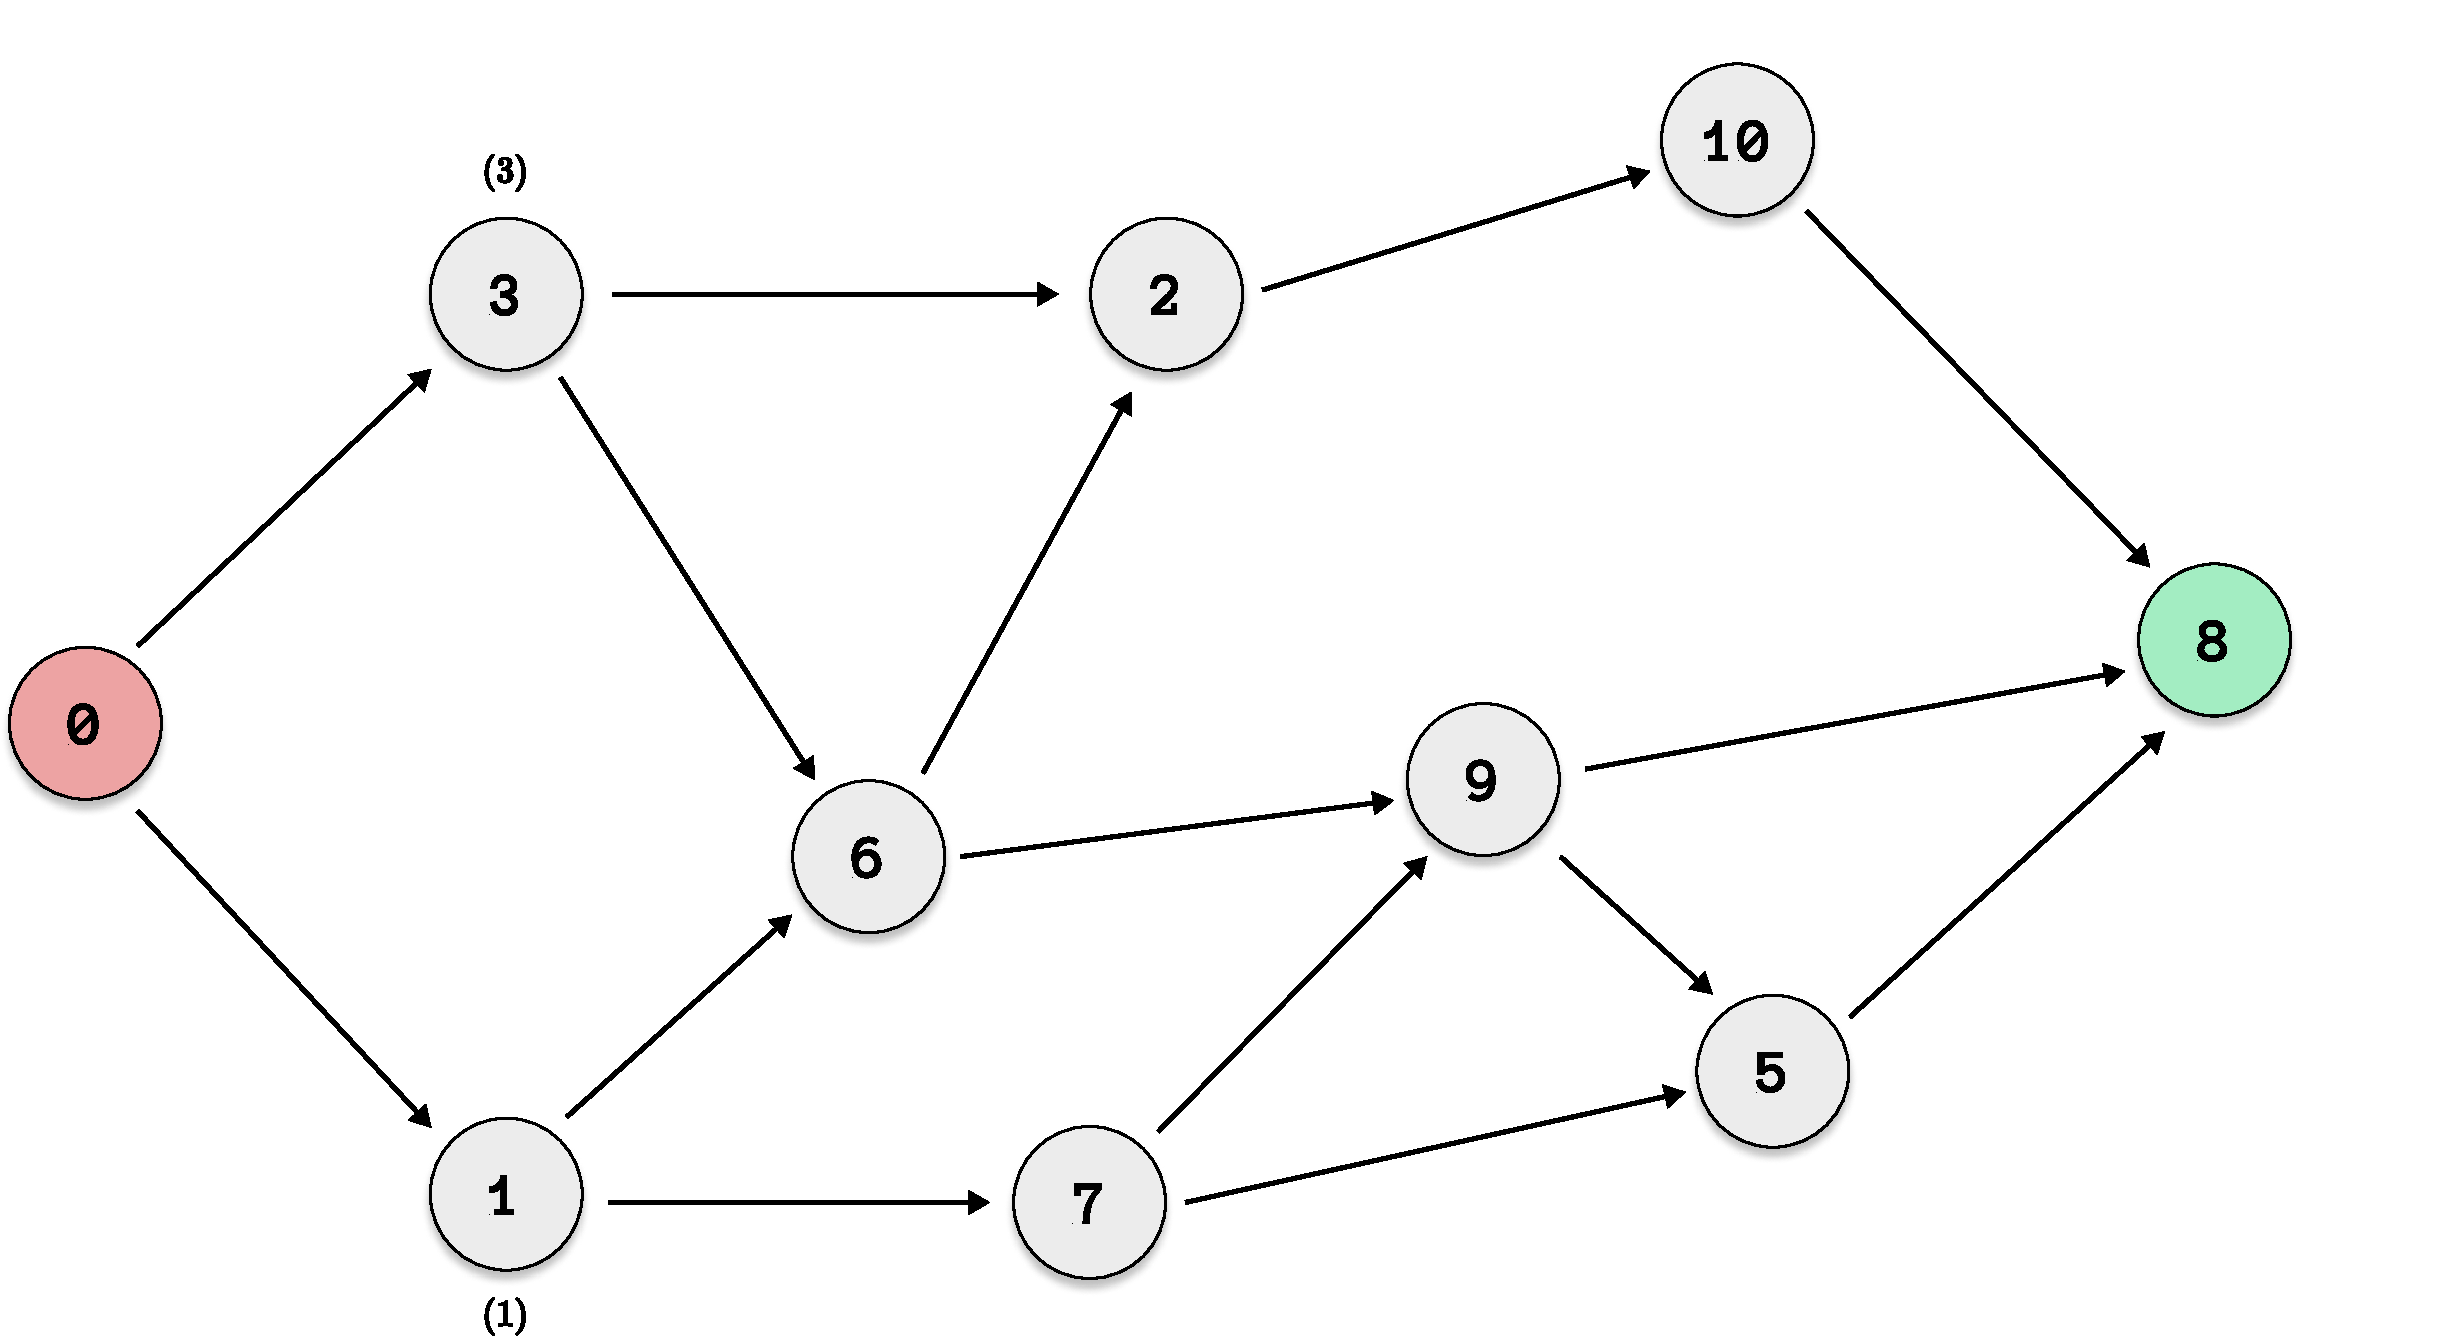
\includegraphics[width=0.85\textwidth]{assets/dag_explicit3.pdf}}
        \only<3>{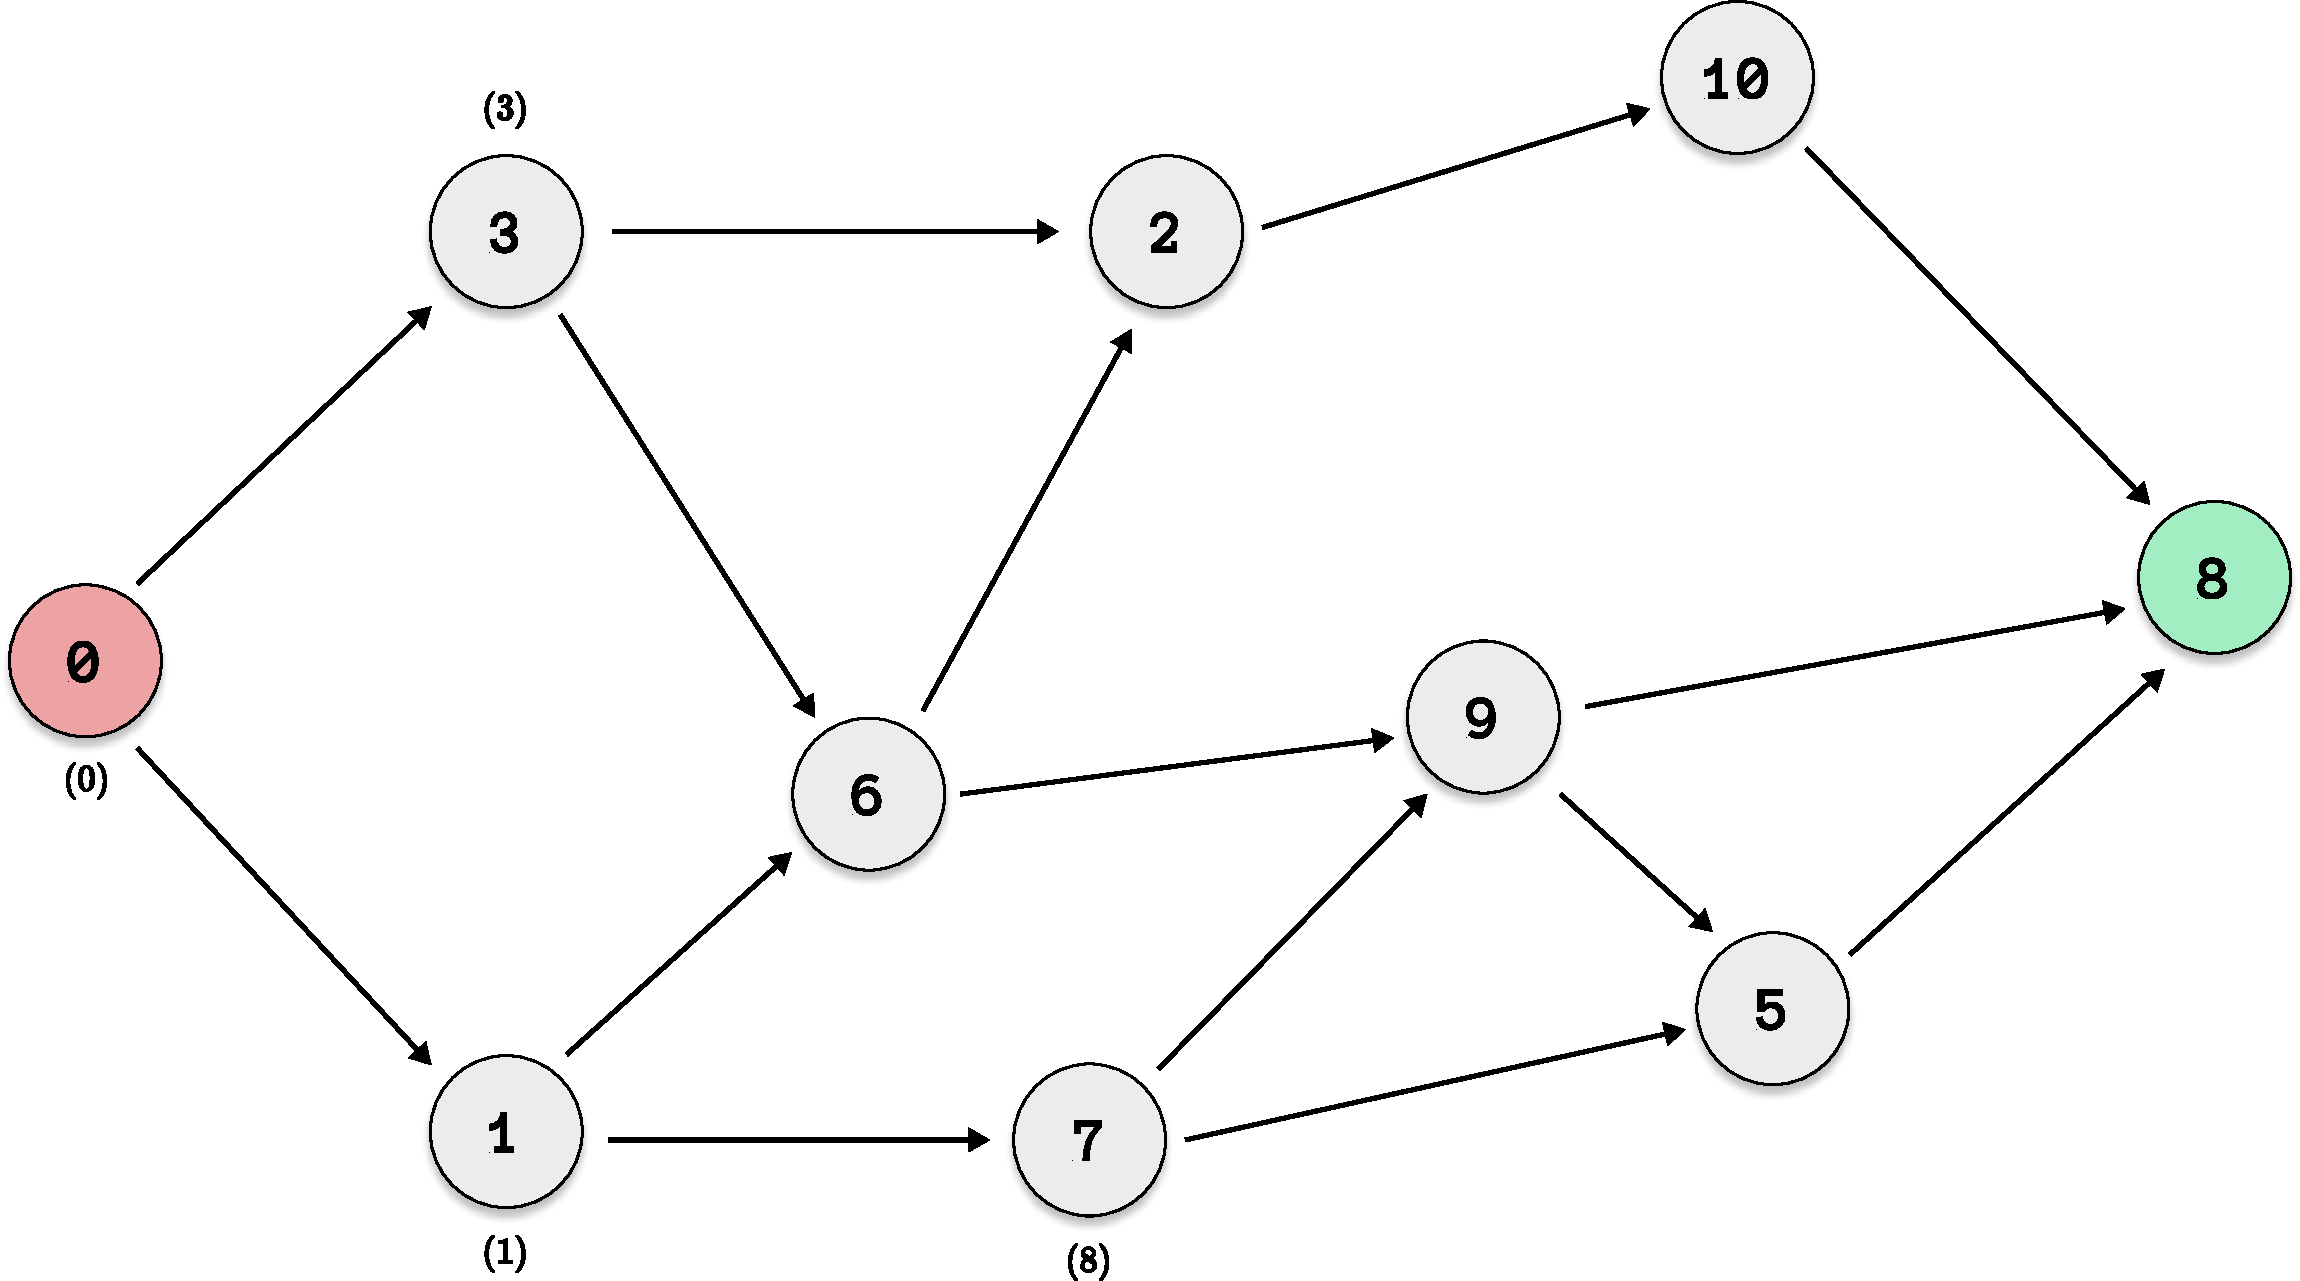
\includegraphics[width=0.85\textwidth]{assets/dag_explicit4.pdf}}
        \only<4>{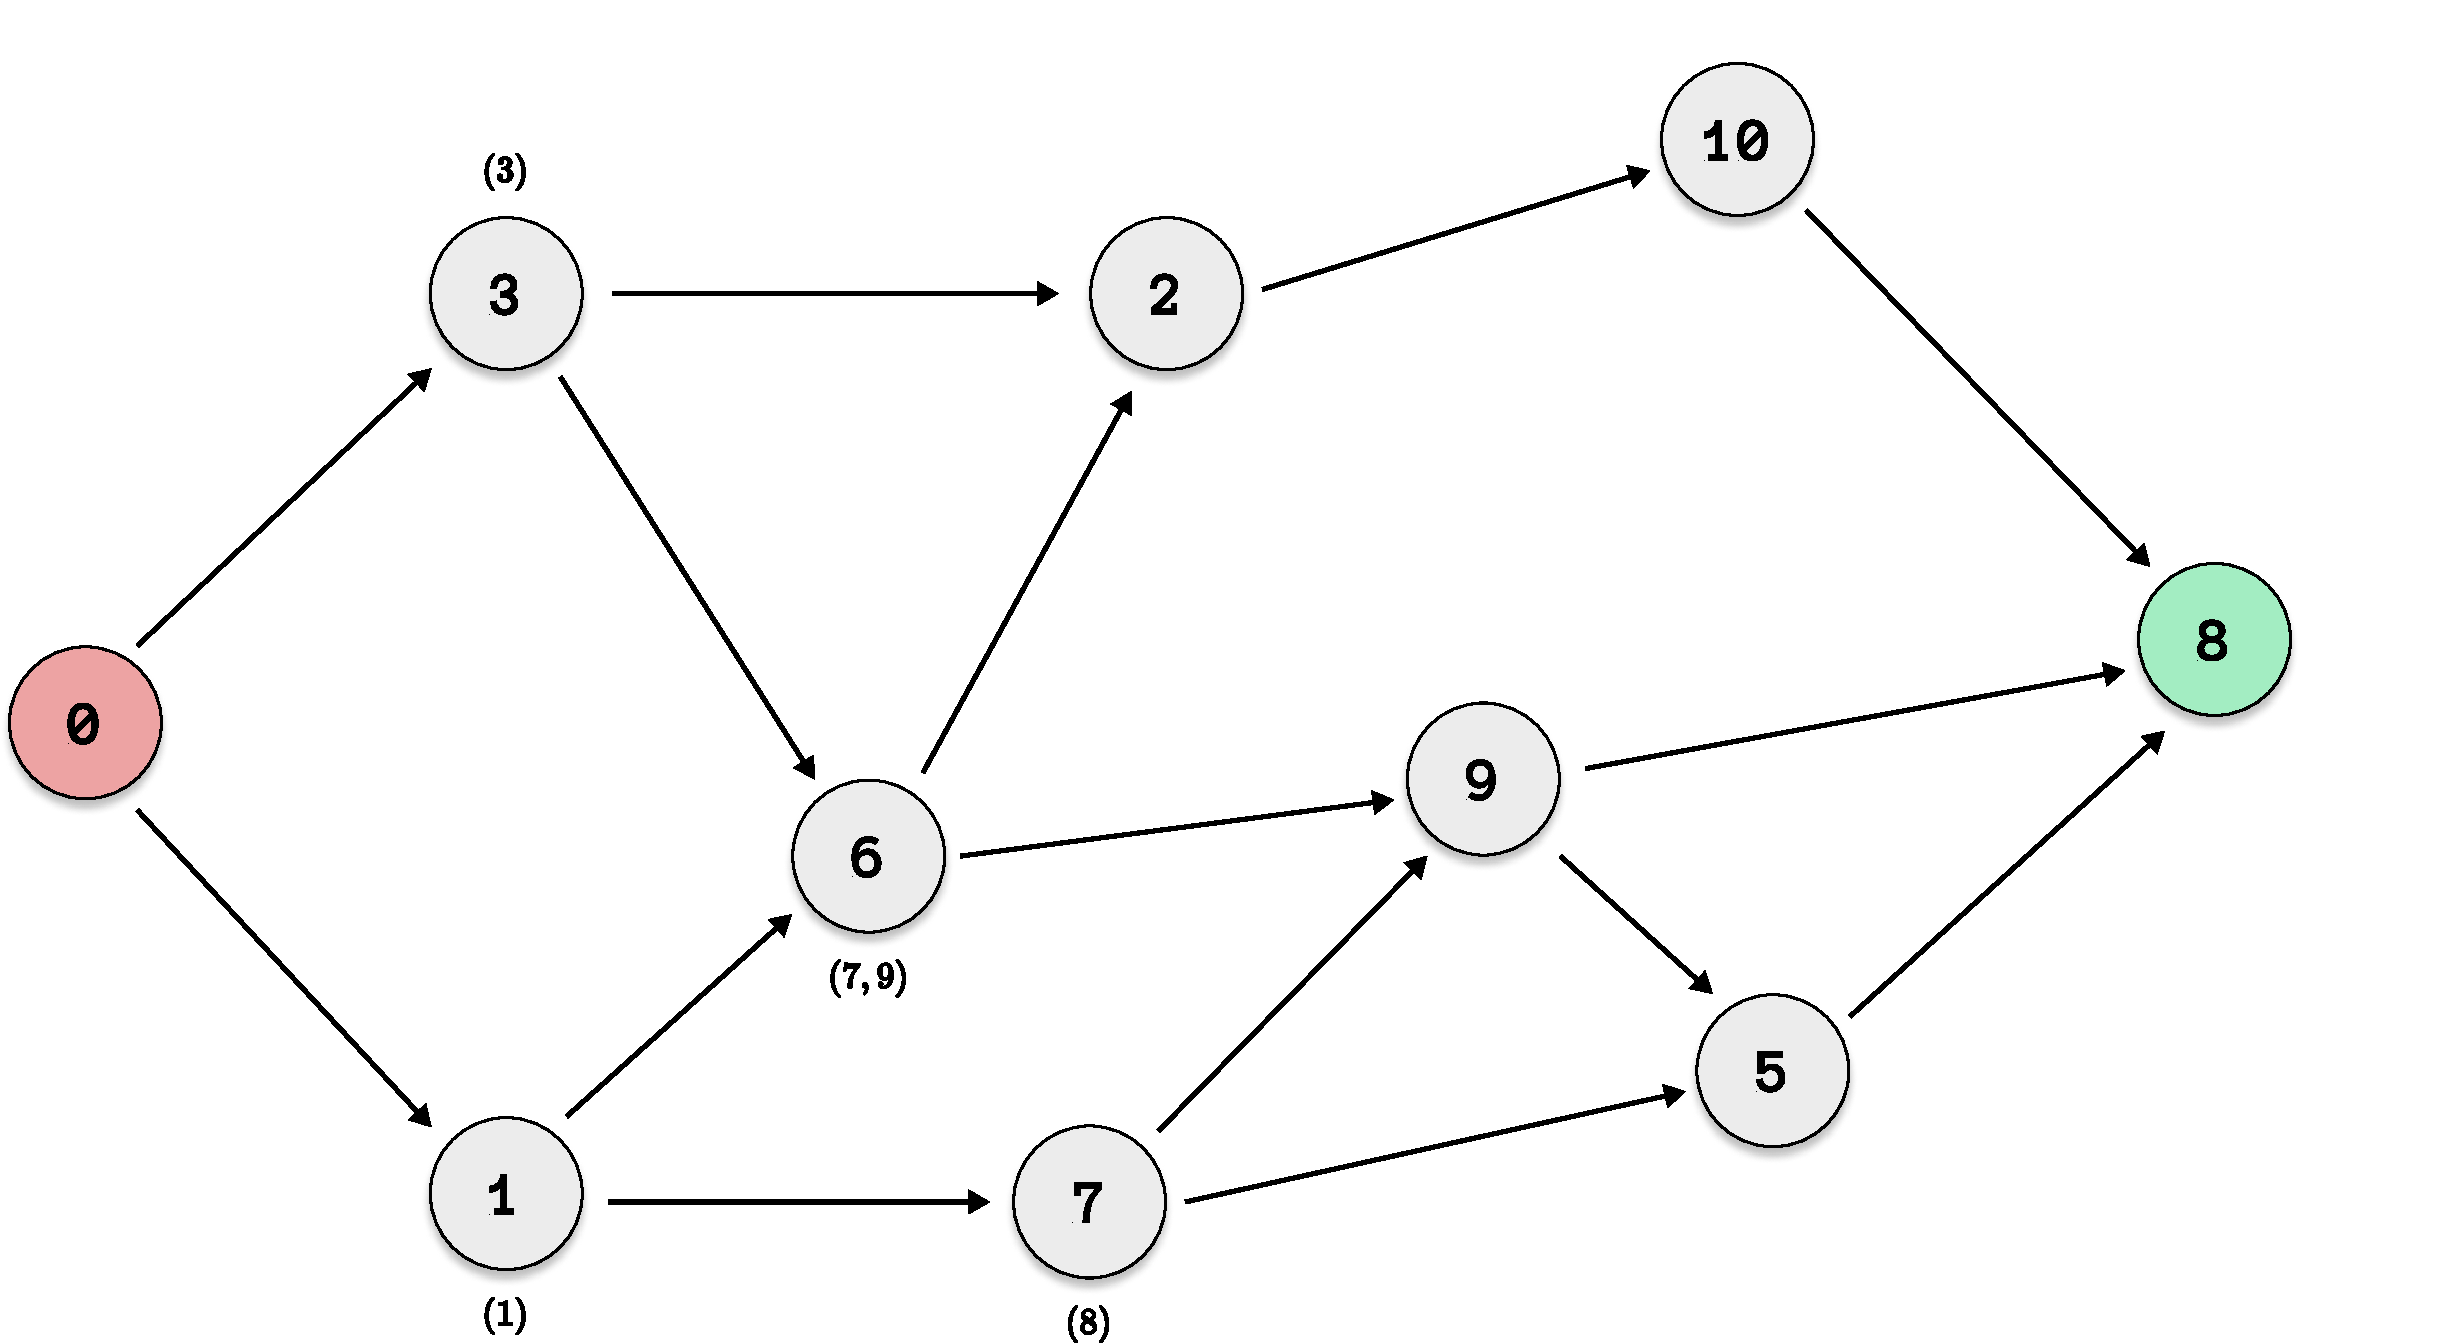
\includegraphics[width=0.85\textwidth]{assets/dag_explicit5.pdf}}
        \only<5>{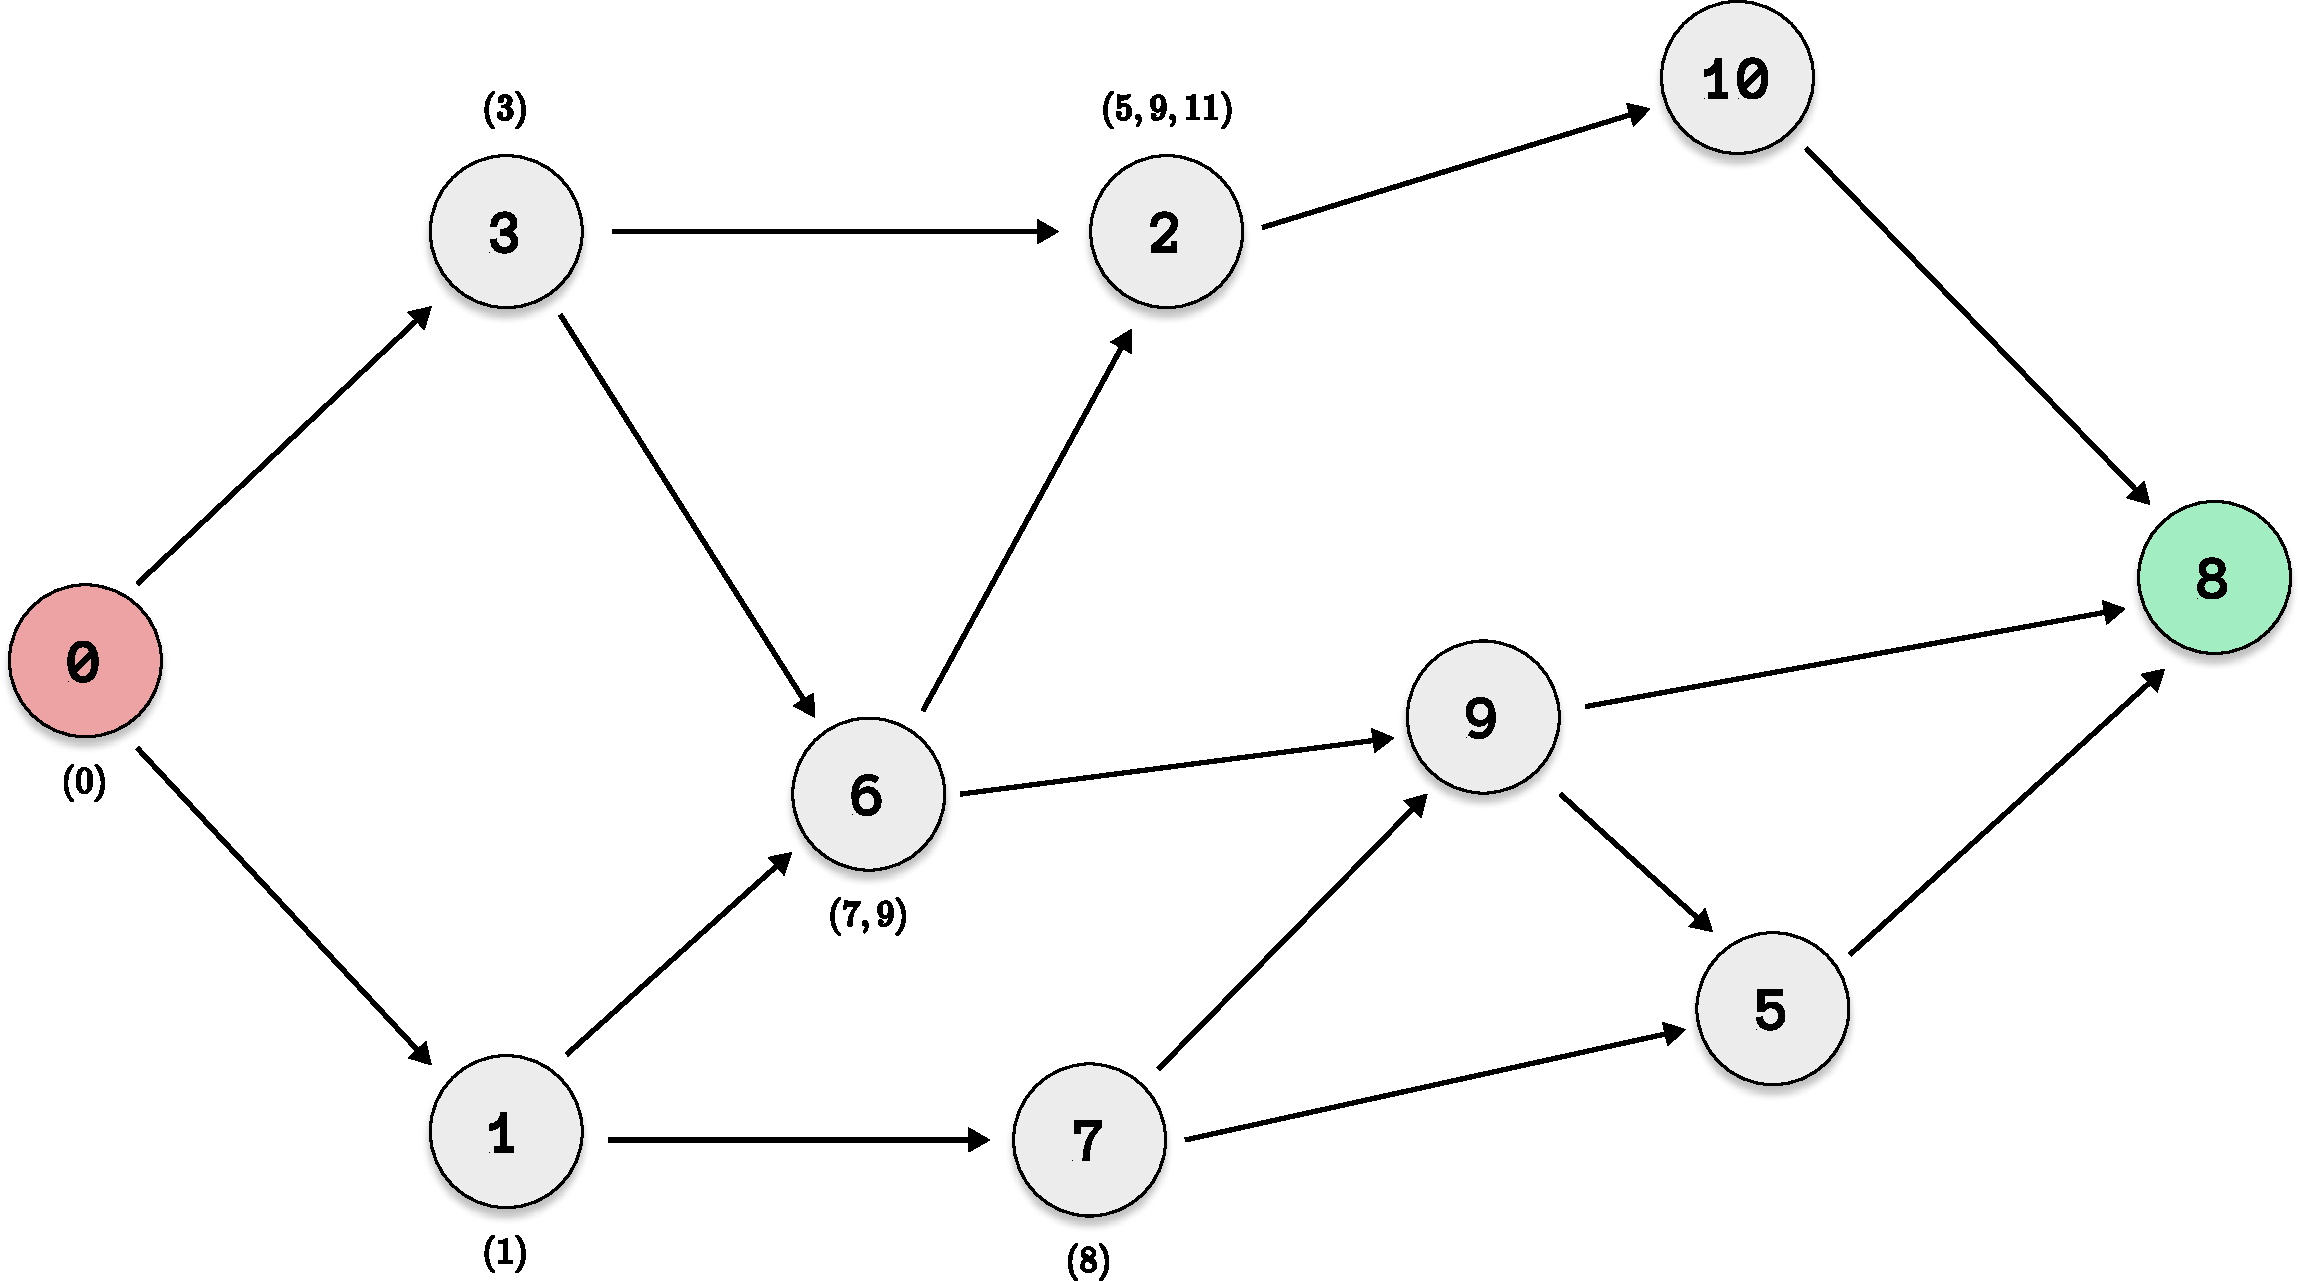
\includegraphics[width=0.85\textwidth]{assets/dag_explicit6.pdf}}
        \only<6>{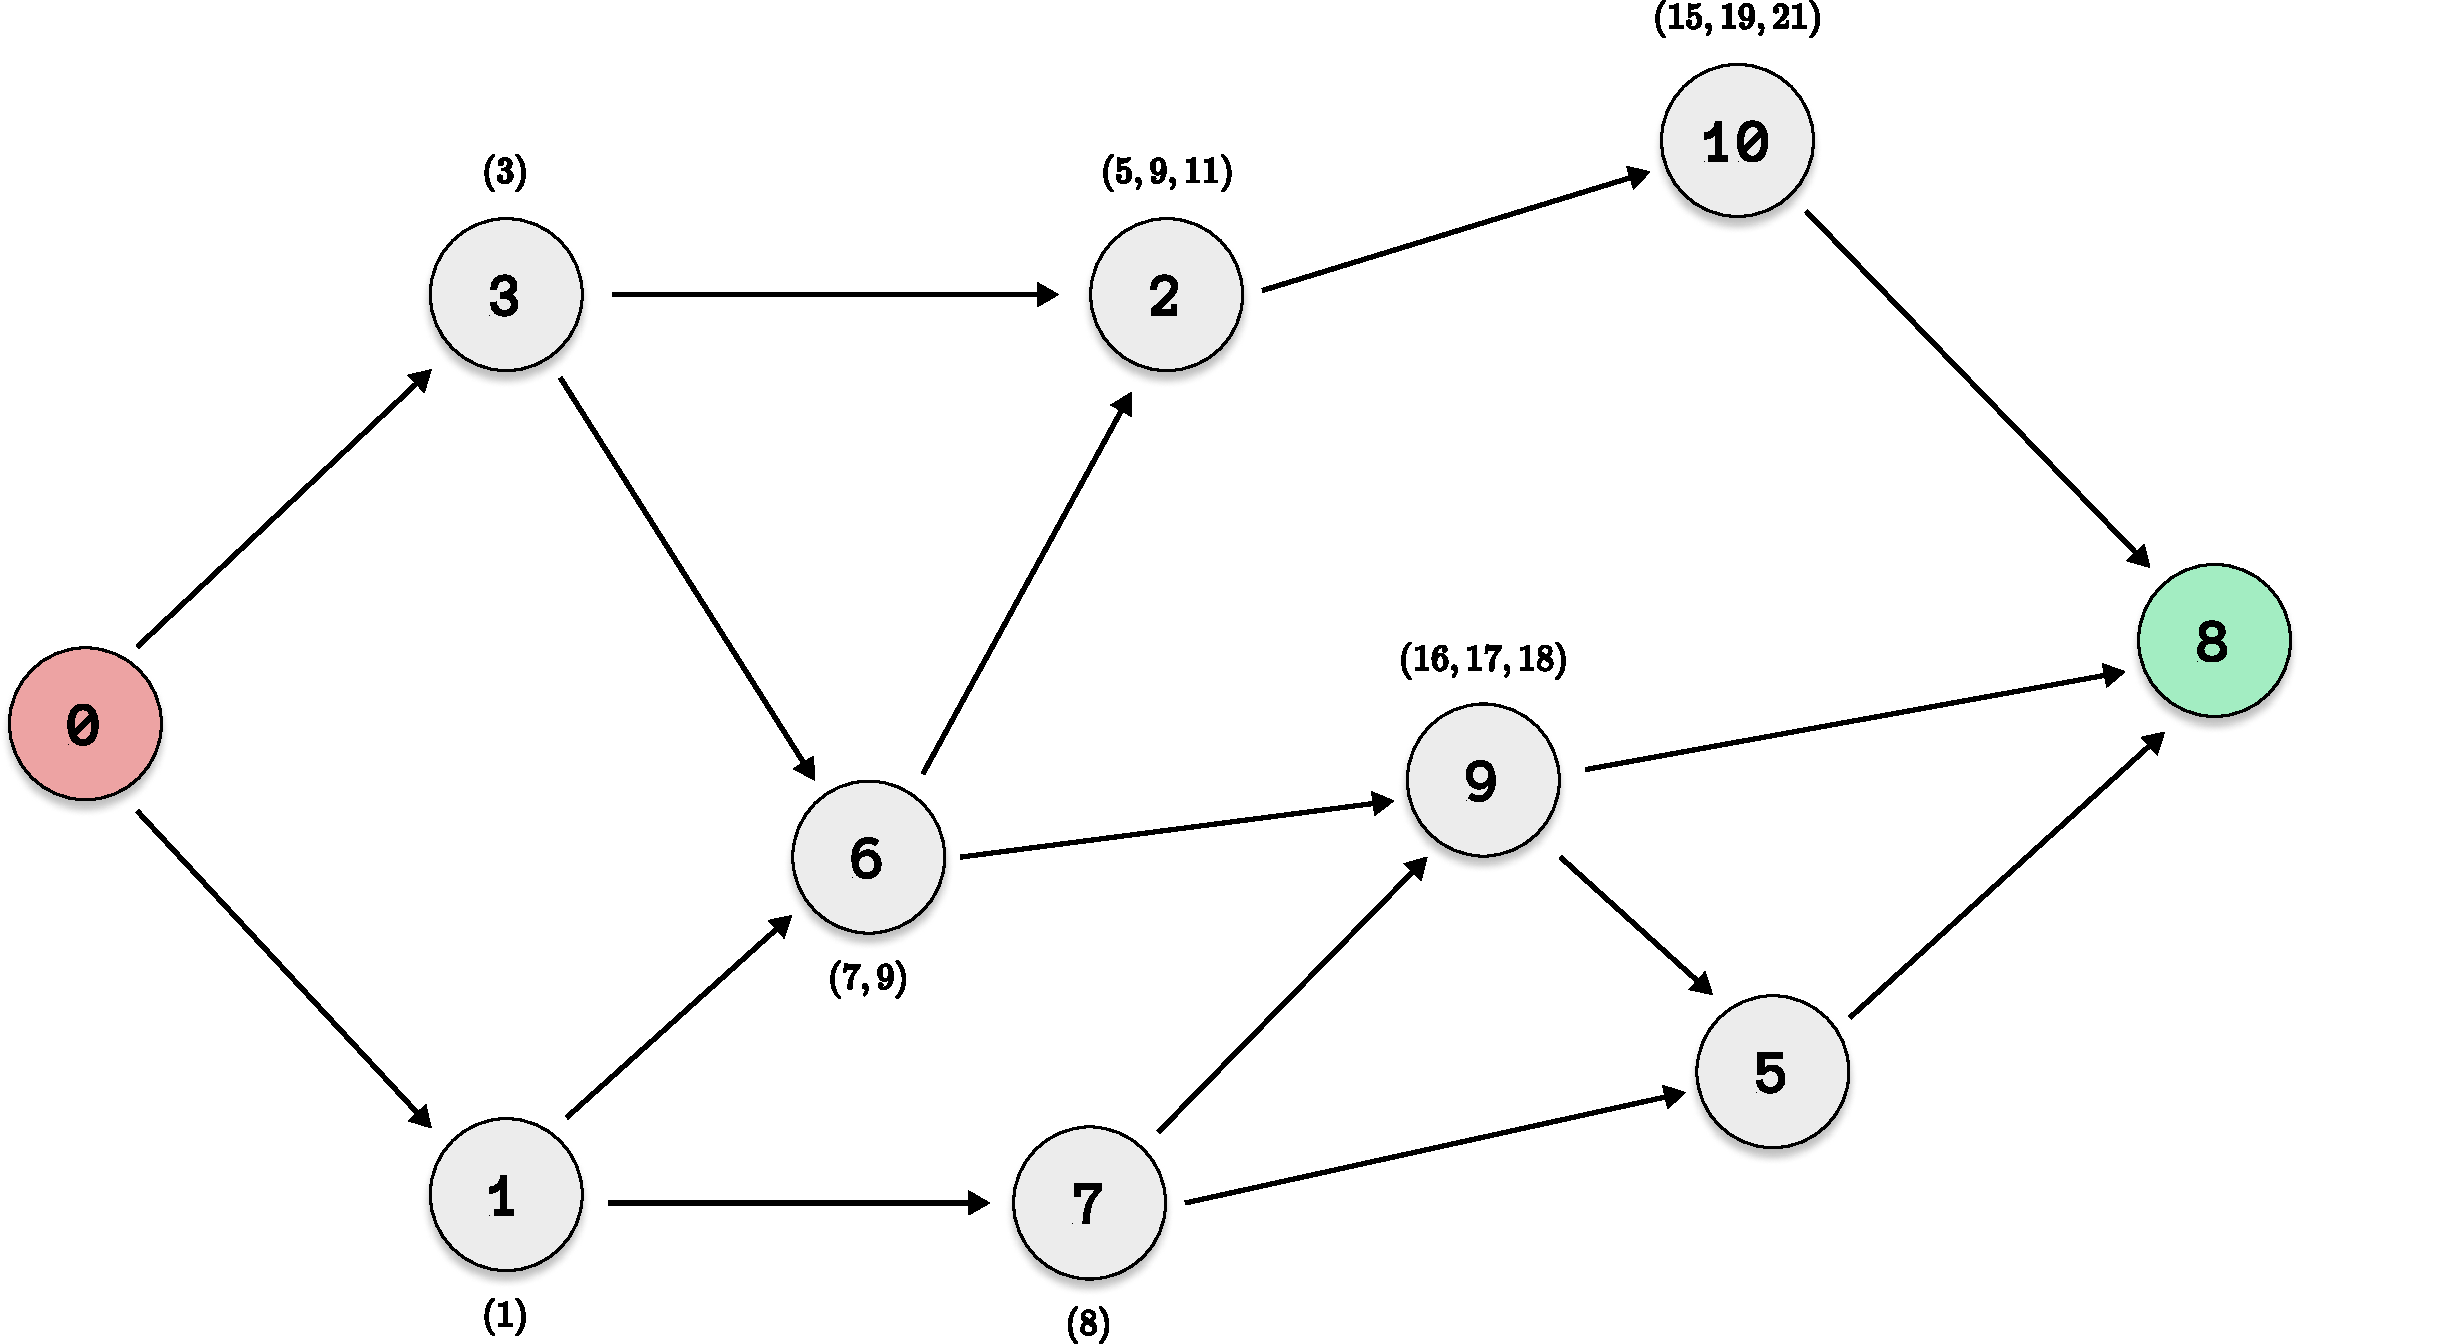
\includegraphics[width=0.85\textwidth]{assets/dag_explicit7.pdf}}
        \only<7>{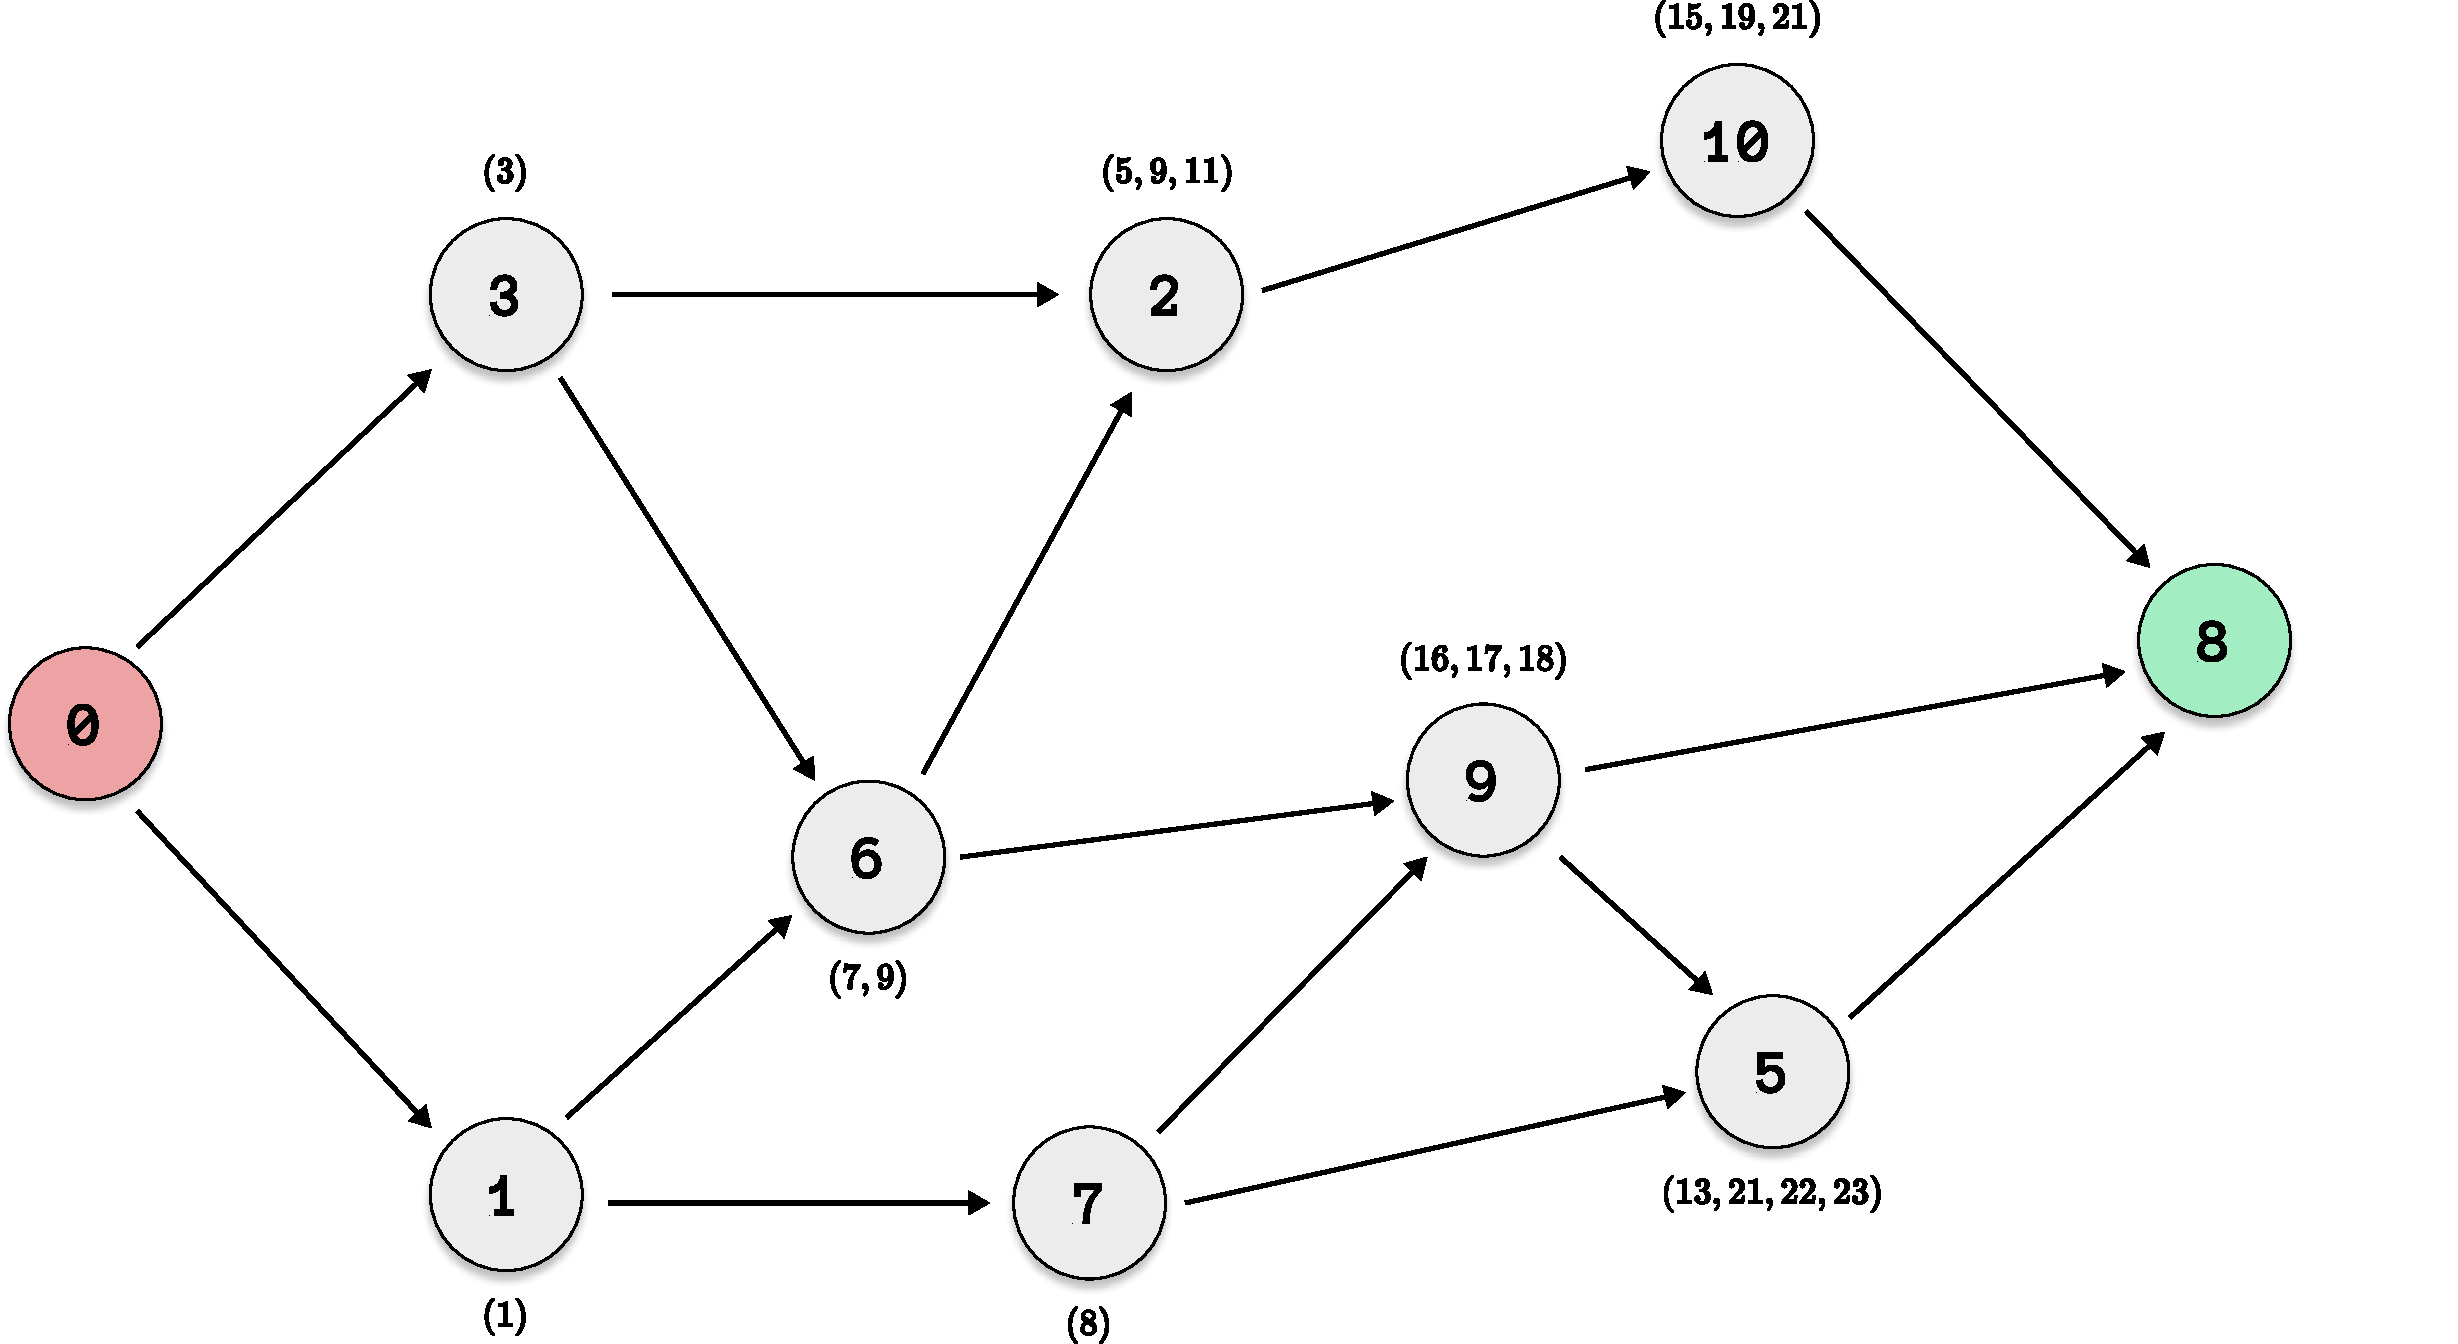
\includegraphics[width=0.85\textwidth]{assets/dag_explicit8.pdf}}
        \only<8>{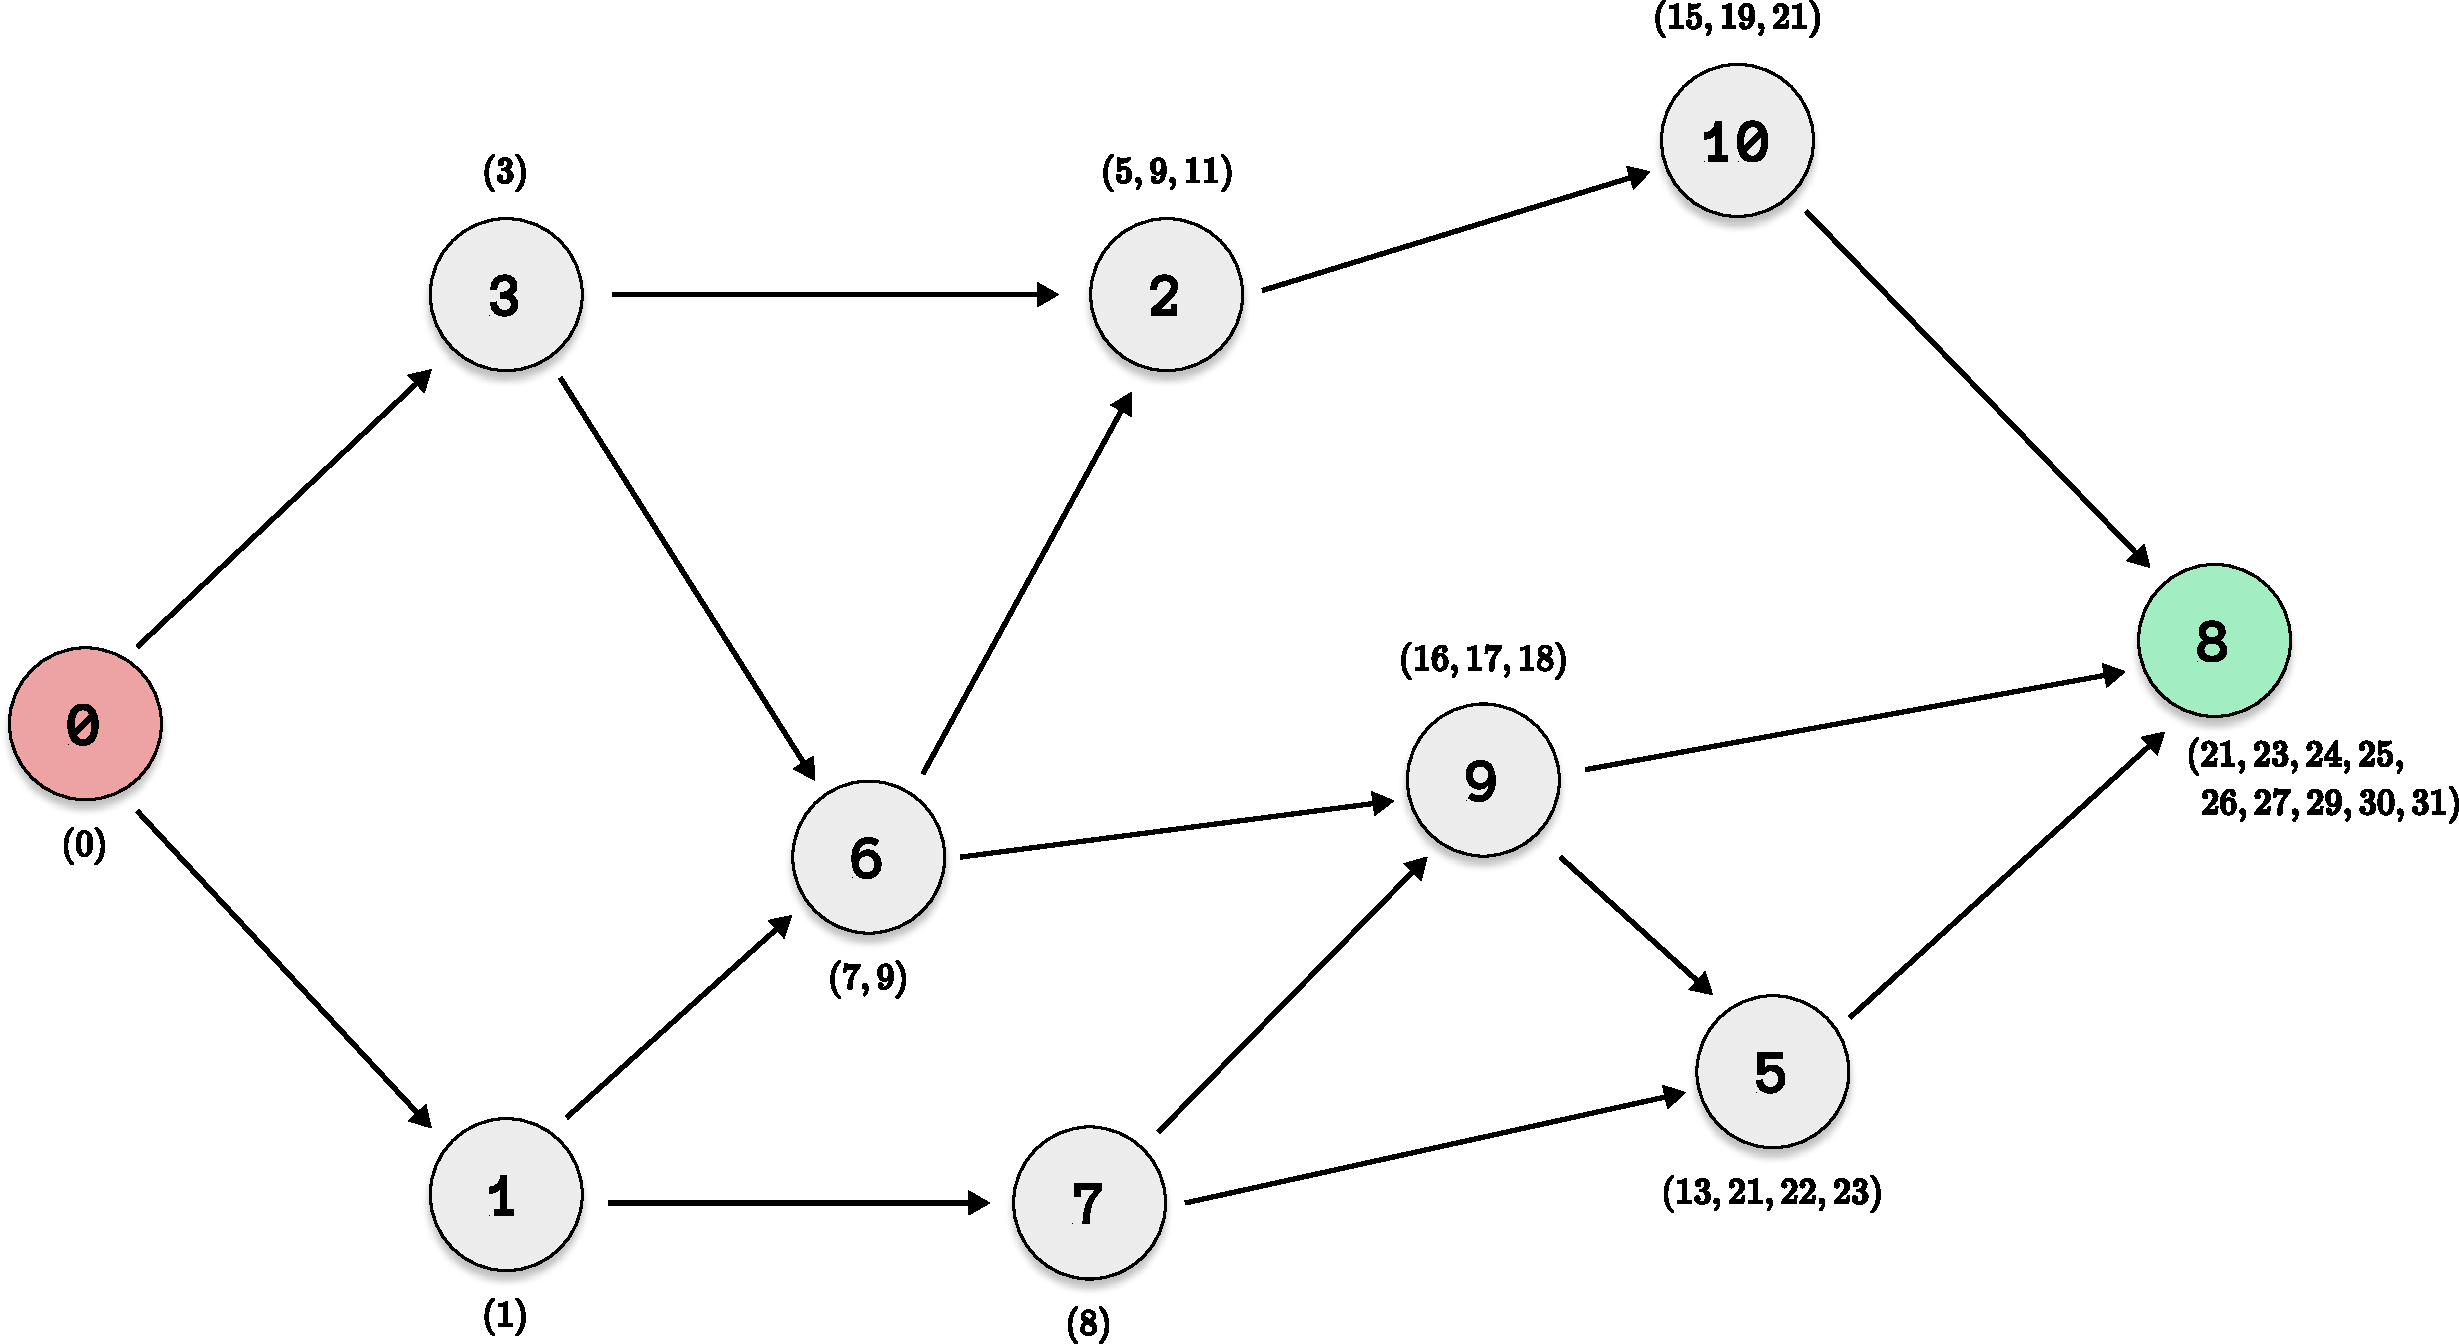
\includegraphics[width=0.85\textwidth]{assets/dag_explicit_final.pdf}}
    \end{figure}
    % \begin{figure}[h!]
    %     \centering
    %     % \resizebox{0.9\textwidth}{!}{% Reduced size slightly to make space for labels
    %     %     \begin{tikzpicture}[
    %     %         node distance=1.5cm and 1cm,
    %     %         base_node/.style={circle, draw=black, thick, minimum size=8mm, inner sep=0pt, font=\sffamily},
    %     %         root_node/.style={base_node, fill=red!60, text=black},
    %     %         % Definizione stile per label O-set
    %     %         data_label/.style={font=\tiny\ttfamily, text=blue!80!black, anchor=north},
    %     %         edge_style/.style={->, >={Stealth[length=2mm]}, thick, draw=black}
    %     %         ]

    %     %         % Nodes (pesi dentro)
    %     %         \node[root_node] (0) at (0, 2) {0};
    %     %         \node[base_node] (1) at (1.5, 0) {1};
    %     %         \node[base_node] (3) at (1.5, 4) {3};
    %     %         \node[base_node] (6) at (3.5, 1.5) {6};
    %     %         \node[base_node] (7) at (4.5, 0) {7};
    %     %         \node[base_node] (2) at (5.5, 4) {2};
    %     %         \node[base_node] (9) at (6.5, 2) {9};
    %     %         \node[base_node] (5) at (9, 0.5) {5};
    %     %         \node[base_node] (10) at (8.5, 5) {10};
    %     %         \node[base_node] (8) at (11, 3) {8};

    %     %         % Edges
    %     %         \draw [edge_style] (0) -- (1); \draw [edge_style] (0) -- (3);
    %     %         \draw [edge_style] (1) -- (6); \draw [edge_style] (1) -- (7);
    %     %         \draw [edge_style] (3) -- (2); \draw [edge_style] (3) -- (6);
    %     %         \draw [edge_style] (6) -- (2); \draw [edge_style] (6) -- (9);
    %     %         \draw [edge_style] (7) -- (5); \draw [edge_style] (7) -- (9);
    %     %         \draw [edge_style] (2) -- (10);
    %     %         \draw [edge_style] (9) -- (5); \draw [edge_style] (9) -- (8);
    %     %         \draw [edge_style] (10) -- (8); \draw [edge_style] (5) -- (8);

    %     %         % O-Set Labels appearing step-by-step
    %     %         \node<1->[data_label, red] at (0.south) {\{0\}};
    %     %         \node<2->[data_label] at (1.south) {\{1\}};
    %     %         \node<2->[data_label] at (3.south) {\{3\}};
    %     %         \node<3->[data_label] at (7.south) {\{8\}};
    %     %         \node<4->[data_label] at (6.south) {\{7, 9\}};
    %     %         \node<5->[data_label] at ([xshift=0.3cm]2.south) {\{5, 9, 11\}};
    %     %         \node<6->[data_label] at ([yshift=-0.1cm, xshift=0.2cm]9.south) {\{16, 17, 18\}};
    %     %         \node<7->[data_label] at (10.south) {\{15, 19, 21\}};
    %     %         \node<8->[data_label] at (5.south) {\{13, 21, 22, 23\}};
    %     %         \node<9->[data_label, align=center] at ([yshift=-0.2cm, xshift=0.4cm]8.south) {\{21, 23, 24, 25, \\ 26, 27, 29, 30, 31\}};

    %     %     \end{tikzpicture}
    %     % } % End resizebox
    % \end{figure}
\end{frame}

% --- SLIDE 12: The Rank Query - Concept ---
\begin{frame}{The Rank Query on Weighted DAGs}
    \framesubtitle{What Values are "Active" at Node N?}
    % \begin{block}{Motivation}
    %     The $\mathcal{O}$-Set ($\mathcal{O}_N$) tells us the \alert{final} path weights ending at node $N$.
    %     But we want to know which cumulative weight values are relevant \alert{during} the "processing" step associated with node $N$ itself.
    % \end{block}
    \begin{block}{Rank Query on a Node $N$: $\mathrm{rank}_G(N)$}
        \begin{enumerate}
            \item Returns a representation of a set of integers derived from the $\mathcal{O}$-set $\mathcal{O}_N$.
                  \[ S_N = \bigcup_{x \in \mathcal{O}_N} \{ z \in \mathbb{N}_0 \mid \max(0, x - w(N) + 1) \le z \le x \}. \]
                  \vspace{-1em}
                  \pause
            \item These intervals are then maximally merged. The query $\mathrm{rank}_G(N)$ returns a \alert{minimal collection of disjoint closed integer intervals}
                  \[ \mathcal{R}_N = \{[l_1, r_1], [l_2, r_2], \dots, [l_p, r_p]\} \]
                  such that their union exactly covers $S_N$.
                  % \item Return the result as a \alert{minimal set of disjoint intervals} $\mathcal{R}_N$.
        \end{enumerate}
    \end{block}
    $\mathcal{R}_N$ captures the range of possible cumulative sums during the \emph{activity} at node $N$

\end{frame}

% --- SLIDE 13: The Challenge: Storing Path Information ---
\begin{frame}{The Challenge: Storing Path Information}
    \framesubtitle{$\mathcal{O}$-Sets Can Be Huge!}

    % Problema e Domanda rimangono uguali
    \begin{itemize}
        \item \textbf{Problem}: The size $|\mathcal{O}_v|$ can grow very large!
        \item \textbf{Question:} Can we represent the necessary information more compactly?
    \end{itemize}


    \begin{alertblock}<2->{Core Idea: Partitioning + Indirection}
        Partition vertices $V$ into two types:
    \end{alertblock}
    \vspace{-1em}
    \begin{columns}[T] % T allinea al top
        \begin{column}{0.48\textwidth}
            \begin{block}<2->{1. Explicit Vertices ($V_E$)}
                \centering
                Store $\mathcal{O}_v$ directly. \\
                (\textit{Simple, but potentially large})
            \end{block}
            % \uncover<3->{\textbf{}
        \end{column}

        \begin{column}{0.48\textwidth}
            \begin{block}<2->{2. Implicit Vertices ($V_I$)}
                \centering
                Do \emph{not} store $\mathcal{O}_v$ explicitly \\
                (\textit{Reconstruct on-the-fly.})
            \end{block}
            \vspace{0.5em}
        \end{column}
    \end{columns}
    \uncover<3->{\textbf{Reconstruction for $v \in V_I$ using}:
        \begin{itemize}
            \item Designated Successor $\sigma(v)$
            \item Offset Sequence $\mathcal{J}_v$ (at $v$)
        \end{itemize}
    }
\end{frame}

% --- SLIDE 14: Successor Choice and Offset Sequence ---
\begin{frame}{Implicit Reconstruction: Successor \& Offset}
    \framesubtitle{How $V_I$ Nodes Refer to Others}

    \begin{block}{1. Designated Successor $\sigma(v)$ (for $v \in V_I$)}
        Which successor should $v$ point to?
        \textbf{Heuristic}: Choose $u = \sigma(v)$ that minimizes $|\mathcal{O}_u|$.
        \[ \sigma(v) \in \underset{u \in Succ(v)}{\operatorname{argmin}} \{ |\mathcal{O}_u| \}. \]
    \end{block}
    \begin{block}{2. Offset Sequence $\mathcal{J}_v$ (for $v \in V_I$)}
        How to get $\mathcal{O}_v$ from $\mathcal{O}_{\sigma(v)}$? Let $u=\sigma(v)$.
        \begin{itemize}
            % \item Property: We know $|\mathcal{O}_v| \le |\mathcal{O}_u|$.
            \item \textbf{Relationship}: Each element $x_k \in \mathcal{O}_v$ comes from some $y_{j_k} \in \mathcal{O}_u$ via $x_k = y_{j_k} - w(u)$.
            \item \textbf{Offset Sequence $\mathcal{J}_v$}: Stores the index $j_k$ corresponding to each $x_k$.
                  \[ \mathcal{J}_v = (j_0, j_1, \dots, j_{m-1}), \quad \text{where } m = |\mathcal{O}_v| \]
        \end{itemize}
    \end{block}

\end{frame}

% --- SLIDE 15: Example: Computing O_9[1] (Static Structure First) ---
\begin{frame}{Example: Computing $\mathcal{O}_9[1]$}
    \framesubtitle{Following the Successor Path: $9 \to 5 \to 8$}
    \begin{figure}[hbtp]
        \centering
        % Replace TikZ with sequential images
        \only<1>{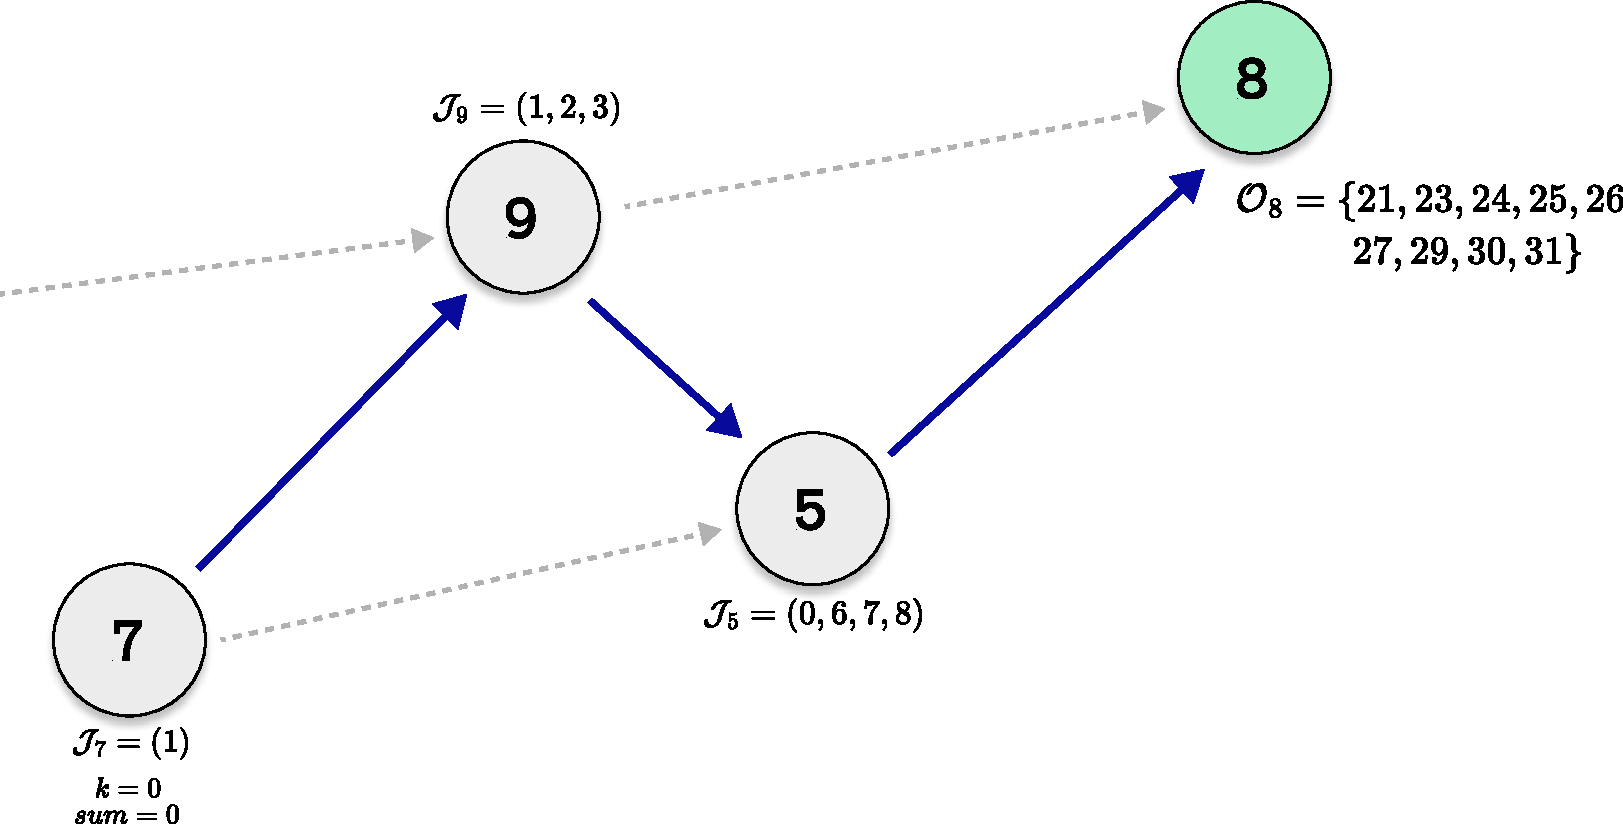
\includegraphics[width=0.9\textwidth]{assets/dag_query1.pdf}}
        \only<2>{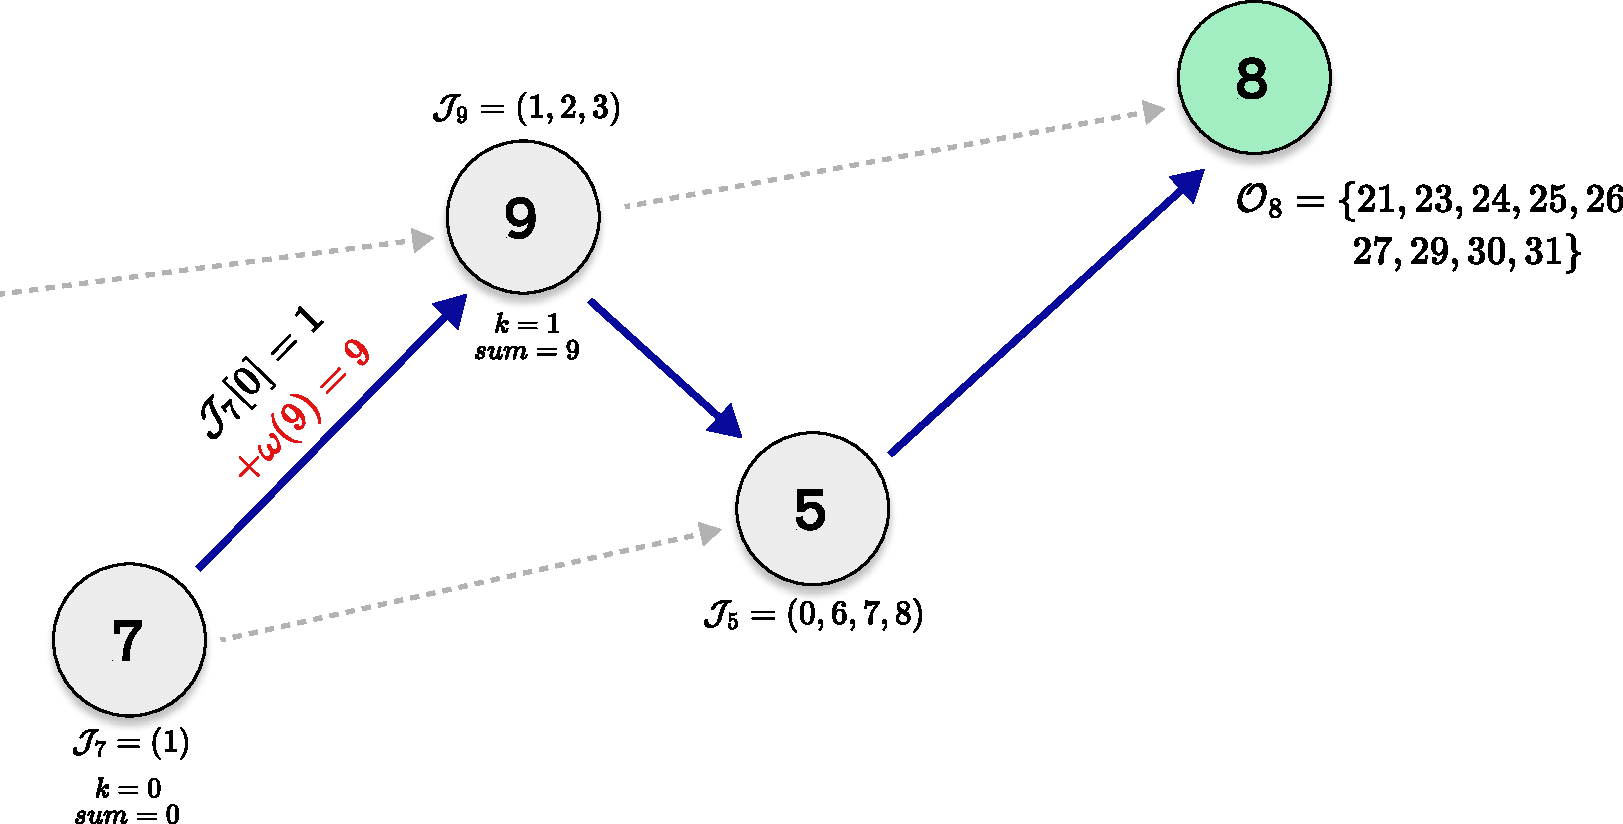
\includegraphics[width=0.9\textwidth]{assets/dag_query2.pdf}}
        \only<3>{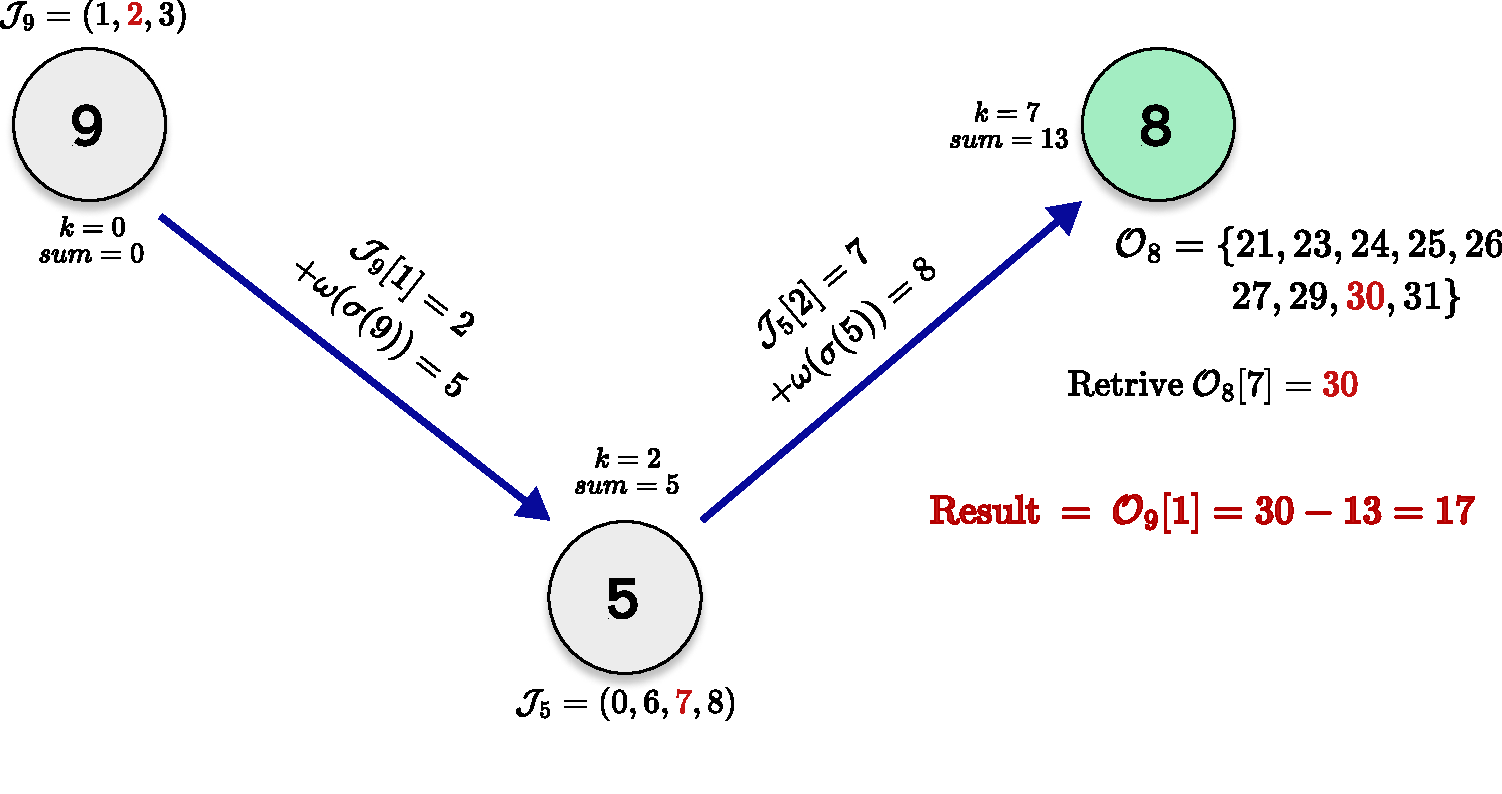
\includegraphics[width=0.9\textwidth]{assets/dag_query3.pdf}}
        % \only<4>{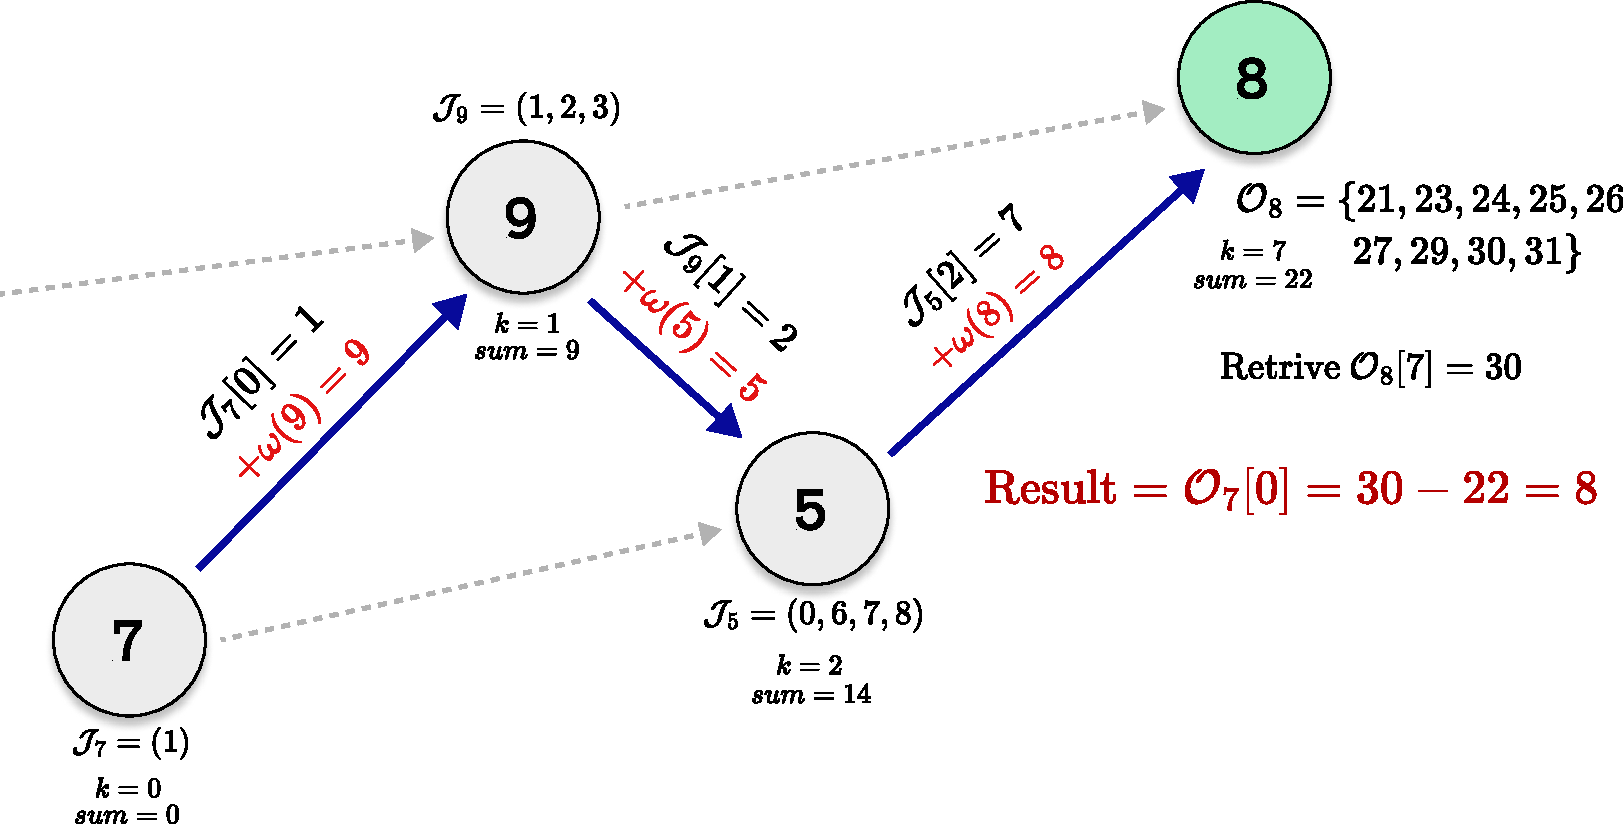
\includegraphics[width=0.9\textwidth]{assets/dag_query4.pdf}}
    \end{figure}
\end{frame}

% --- SLIDE 16: Example: Computing O_7[0] (Dynamic Structure) ---
\begin{frame}{Succinct Data Structure: Components}
    \framesubtitle{Arrays Indexed by Vertex ID}
    % divide in two columns
    \begin{columns}[T]
        \column{0.5\textwidth}
        \uncover<1->{\begin{center}
                \textbf{Each node stores 3 components}
            \end{center}
            \begin{center}
                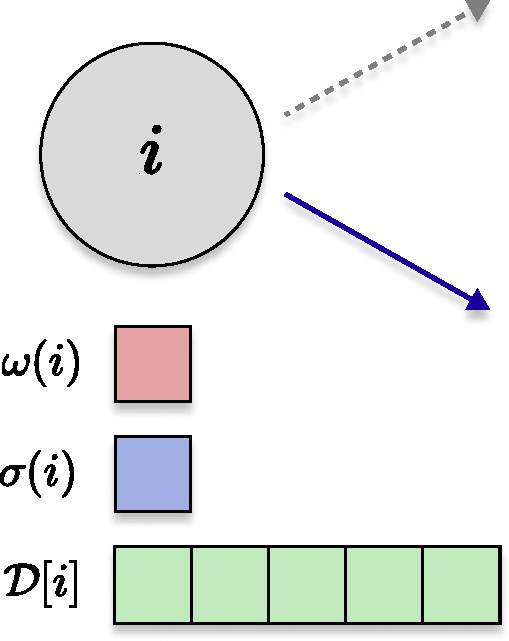
\includegraphics[width=0.55\textwidth]{assets/AoS.pdf}
            \end{center}}

        \column{0.5\textwidth}
        \uncover<2->{\begin{center}
                \textbf{Succinct DAG as a Struct of Arrays}
            \end{center}
            \begin{center}
                \vspace{0.5em}
                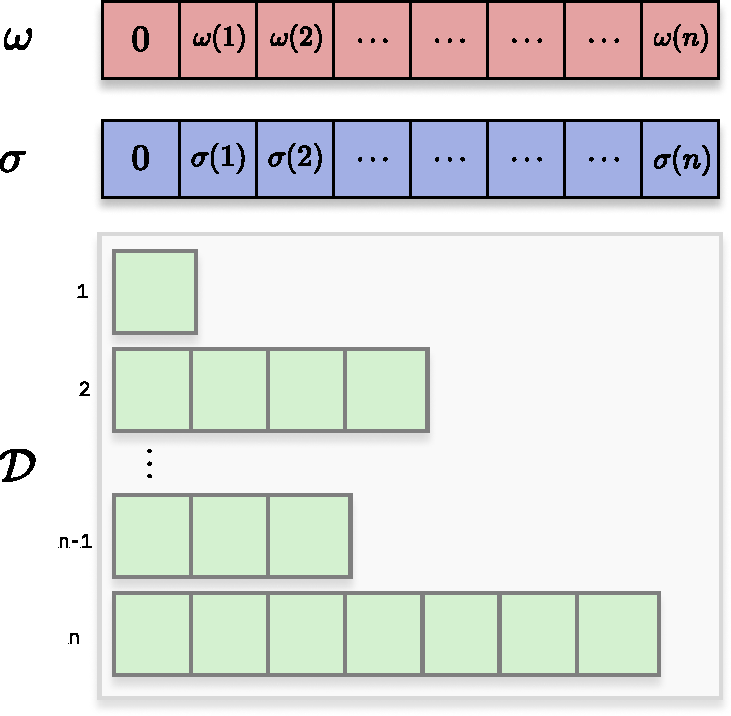
\includegraphics[width=0.8\textwidth]{assets/SoA.pdf}
            \end{center}}
    \end{columns}
\end{frame}

% --- SLIDE 17: Compression Strategies - Overview ---
\begin{frame}{Compression Strategies}
    \framesubtitle{Reducing Memory Footprint}
    \begin{center}
        \begin{tabular}{l l}
            \toprule
            \textbf{Component}              & \textbf{Description}                             \\
            \midrule
            % Le prime due righe appaiono insieme al passo 1
            \uncover<1->{%
            $\mathcal{W}$ (Node weights)    & Array of positive integers.                      \\
            } % Appare dalla slide 1 in poi
            \uncover<1->{%
            $\Sigma$ (Successor IDs)        & Array of positive integers.                      \\
            } % Appare dalla slide 1 in poi
            % L'ultima riga e la linea inferiore appaiono al passo 3
            \uncover<3->{%
            $\mathcal{D}$ (Associated Data) & Array of arrays of increasing positive integers. \\
                \bottomrule
            } % Appare dalla slide 3 in poi
        \end{tabular}
    \end{center}
    \vspace{-1.5em}
    % Il blocco alert appare al passo 2, insieme ai primi due item
    \begin{alertblock}{Compression Options}<2-> % Appare dalla slide 2 in poi
        \begin{itemize}
            % I primi due item appaiono al passo 2
            \item<2-> Variable-Length Integer Coding $\longrightarrow$ we published a Rust library\footnote[1]{\url{https://crates.io/crates/compressed-intvec}} for this! % Appare dalla slide 2 in poi
            \item<2-> Wavelet Trees \emph{(for nodes with small weight range)} % Appare dalla slide 2 in poi
                % Gli ultimi due item appaiono al passo 4
            \item<4-> Elias-Fano Encoding \emph{(for monotonic sequences)} % Appare dalla slide 4 in poi
            \item<4-> Run-Length Encoding (RLE) \emph{(for clustered monotonic sequences)} % Appare dalla slide 4 in poi
        \end{itemize}
    \end{alertblock}
\end{frame}

% --- SLIDE 18: Baseline: Graph Entropy H0(G) ---
\begin{frame}{Space Efficiency: Baseline Comparison}
    \framesubtitle{How Much Information is in the Graph?}
    To evaluate our structure's space, \alert{we need a baseline}.
    \begin{block}<1->{$0^{th}$-Order Graph Entropy $H_0(G)$}
        A theoretical lower bound for storing the \emph{entire} weighted DAG ($V, E, w$) losslessly.
        \[ H_0(G) = \underbrace{H_W(G)}_{\text{Cost for Weights}} + \underbrace{H_E(G)}_{\text{Cost for Topology (Edges)}} \]
    \end{block}
    \begin{itemize}
        \item<2-> $H_W(G) \approx \sum_{v \in V} \log(w(v)+1)$ bits (\emph{Minimal binary encoding for weights}).
        \item<3-> $H_E(G) \approx \log \binom{n(n-1)}{m}$ bits (\emph{Cost to choose $m=|E|$ edges out of all possible $n(n-1)$}).
    \end{itemize}
    \vspace{0.5em}
    \uncover<4->{\textbf{Any method saving the \emph{full} graph structure needs at least $H_0(G)$ bits!}}

\end{frame}

% --- SLIDE 19: Space Comparison - Key Numbers ---
\begin{frame}{Space Comparison: Succinct Structure vs. Baselines}
    \framesubtitle{Bitcoin DAG Example ($n \approx 22k, m \approx 50k$)}
    \begin{columns}[c] % Keep [t] for top alignment
        \begin{column}{0.5\textwidth} % Adjusted width potentially
            \centering
            \begin{tabular}{l r}
                \toprule
                \textbf{Method}                       & \textbf{Estimated Bits}          \\
                \midrule
                \textbf{Theoretical Lower Bound}      & \uncover<1->{\textbf{1,525,730}} \\
                \quad Weights $H_W(G)$                & \uncover<1->{60,824}             \\
                \quad Topology $H_E(G)$               & \uncover<1->{1,464,906}          \\
                \midrule
                \textit{Precomputed Rank Queries:}    &                                  \\
                \quad Explicit Binary Storage         & \uncover<2->{4,854,533}          \\
                \quad Elias-Fano Compressed           & \uncover<2->{2,211,849}          \\
                \midrule
                \textbf{Our Succinct DAG}             & \uncover<3->{\textbf{602,808}}   \\
                \quad Weights $\mathcal{W}$           & \uncover<3->{60,824}             \\
                \quad Successors $\Sigma$             & \uncover<3->{297,700}            \\
                \quad Assoc. Data $\mathcal{D}$ (RLE) & \uncover<3->{244,284}            \\
                \bottomrule
            \end{tabular}
            % Removed \end{center}
        \end{column}
        \begin{column}{0.5\textwidth} % Adjusted width to sum to 1.0
            % \begin{alertblock}<4->{Key Result}
            %     Our structure ($S(G)$) is $\approx$ \textbf{2.5x smaller} than the theoretical lower bound ($H_0(G)$) and $\approx$ \textbf{3.7x smaller} than compressed precomputation.
            % \end{alertblock}
            \begin{alertblock}<4->{Achieving Sub-Entropy Space: How?}
                Our structure is \textbf{lossy} regarding the full graph topology:
                \begin{itemize}
                    \item It \alert{does not store} the complete edge set.
                    \item It only stores the chosen successor $\sigma(v)$ for each implicit node (in $\Sigma$).
                \end{itemize}
                However, it is \textbf{lossless} for computing the specific \alert{Rank Query}.
            \end{alertblock}
        \end{column}
    \end{columns}
\end{frame}
